\chapter{Design of the RV32I Machine}
\label{Chapter3}
	\minitoc
	%\addtocontents{toc}{\protect\contentsline{chapter}{\protect\numberline{}Design of the RV32I Machine}{}{}}
	\vspace{5mm}
	
	In this chapter we will present one by one the CPU's pipeline stages and also the final design. Every part and every module that was created (via $VHDL$) was thoroughly tested before moving to the next one. The whole design consists of five pipeline stages which are the Instruction Fetch, the Instruction Decode, Execute Stage, Memory Stage and Write Back Stage. 
	\clearpage
	
\section{Instruction Fetch - IF}
	 \label{Sec3.1:IF}
	 The Instruction Fetch ($IF$) module consists of a simple memory block (M4K - block)\footnote{The use of M4K was mandatory in our case since we wanted the design to be synthesizable. Having that in mind, the only embedded memory available on our FPGA board was the M4K RAM memory type } that is used to simulate the Instruction Cache (I\$) in our system. 
	 We chose for the I\$ to have $1024$ slots which are $32$-bit wide (since we are implementing a 32-bit architecture). So the total capacitance of the memory is $4096$ B. 
	 
	 \begin{figure}[h!]
	 	\begin{center}
	 		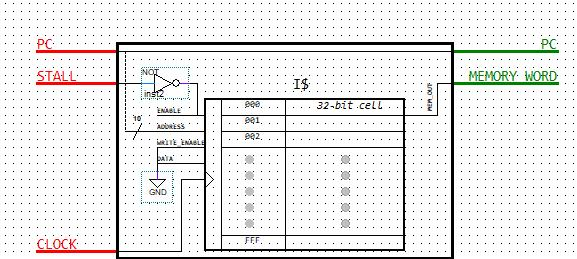
\includegraphics[width=1\textwidth]{IF}
	 		\caption{Instruction Fetch schematic}
	 		\label{Image3.1}
	 	\end{center}
	 \end{figure}
 
	 $IF$ is responsible for fetching the proper instruction ($MEMORY\_WORD$) from I\$. This is done by isolating some bits of the program counter ($PC$) and using them as address for the I\$. Since the memory has $1024$ slots we need $\log_2(1024)=\underline{10}$ bits to iterate through all of them and so, we use the $PC[11..2]$ bits for this work. Last but not least the M4K Memory used was automatically generated by Quartus's II Mega-Wizard Plug-In Manager.	

	\subsection{Module's I/O}
	\label{SubSec3.1.1:I/O}
	 {\small
 	 \renewcommand{\labelenumii}{\Roman{enumii}}
	 \begin{itemize}
	 	\item Inputs:
	 	\begin{enumerate}
	 		
	 		\item \textcolor{red}{$CLOCK$} : System clock.
	 		\item \textcolor{red}{$STALL$} : Pipeline control signal (1-bit).
	 		\item \textcolor{red}{$PC$}    : Program counter (32-bit).
	 	\end{enumerate}
 		\item Outputs:
 		\begin{enumerate}
 		
 			\item \textcolor{forestgreen(web)}{$MEMORY\_WORD$} : Word fetched from I\$ (32-bit).
 			\item \textcolor{forestgreen(web)}{$PC$}	 	   : Program counter (32-bit).
 		\end{enumerate}
	 \end{itemize}}
 	\vspace{5mm}
 	 
 	\clearpage
 	
\section{Instruction Decode - ID}
 	\label{Sec3.2:ID}
 	This is one of the most important and resourceful modules of this design. The Instruction Decode ($ID$) module is responsible for one thing among others; to "recognize" the command that was fetched on the previous cycle and activate all the signals that are needed for the command to be successfully processed.
 	
 	\begin{figure}[h!]
 		\begin{center}
 			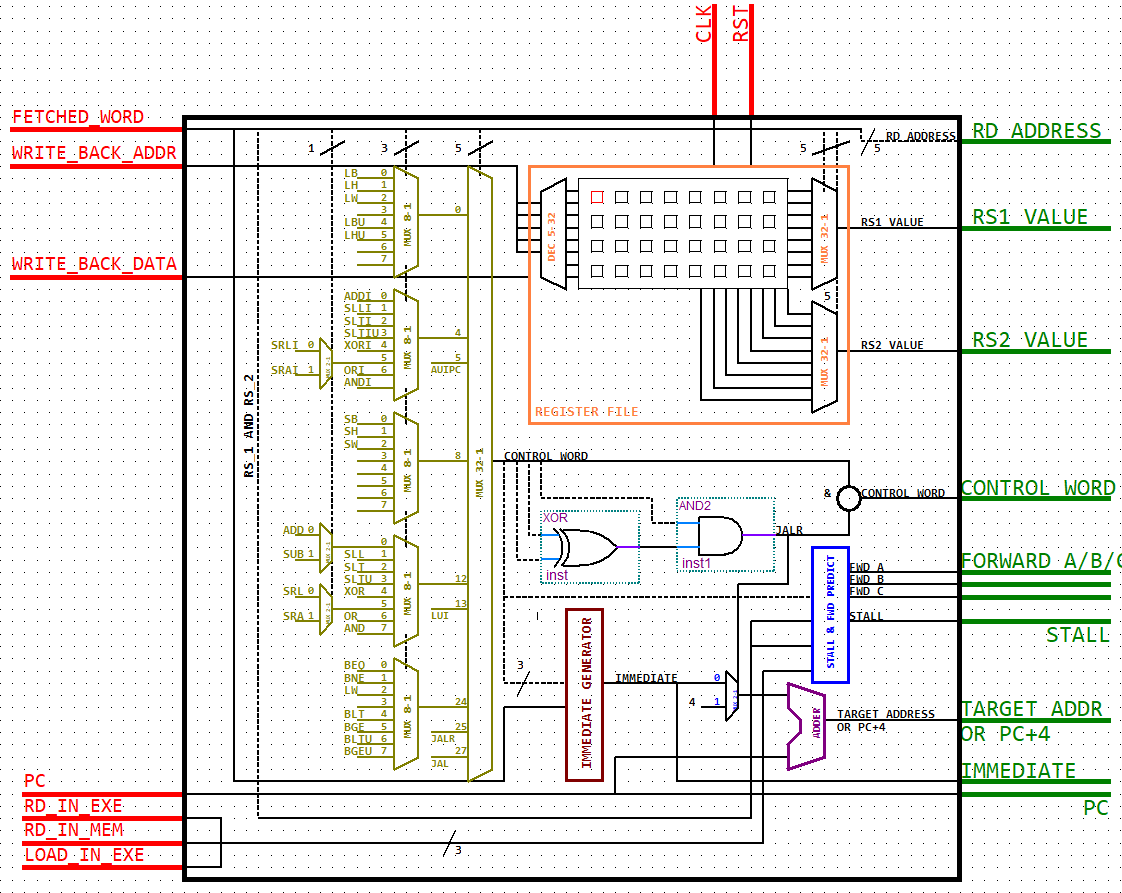
\includegraphics[width=1.0\textwidth]{DECODE}
 			\caption{Instruction Decode schematic}
 			\label{Image3.2}
 		\end{center}
 	\end{figure}
 	
 	\vspace{2mm}
 	
 	Designing the $ID$ module was a trial-and-error process due to the nature of the task that is asserted to it. While being the second part of the pipeline, its development suggests a deep knowledge of what will be done in one, two, and three clock cycles later for every(!) command that is currently being decoded. In this stage we also detect true dependencies ($RAWs$ %sto telos episis
 	) and handle them accordingly to maximize the performance when it is needed. Also, ID is being equipped with a simple \textcolor{byzantium}{Adder} so that it can calculate either the return address of a $JUMP$ or the target address ($PC+IMMEDIATE$) according to the Uncoditional Jump command that is currently being decoded. \\\\
 	Once again, we will follow the color-code of Figure \ref{Image3.2} so one can navigate through the design and the description.
 	
 	\clearpage
 	\subsection{Module's I/O}
 	\label{SubSec3.2.1:I/O}
 	{\small
 		\renewcommand{\labelenumii}{\Roman{enumii}}
 		\begin{itemize}
 			\item Inputs:
 			\begin{enumerate}
 				
 				\item \textcolor{red}{$CLK$} : System clock.
 				\item \textcolor{red}{$RST$} : System reset signal (1-bit). 
 				\item \textcolor{red}{$FETCHED\_WORD$}: Feed from $IF$; word read from I\$ (32-bits). 
 				\item \textcolor{red}{$WRITE\_BACK\_ADDR$}  : Feed from $Write\ Back$ stage; $rd$ register address (5-bits).
 				\item \textcolor{red}{$WRITE\_BACK\_DATA$}	: Feed from $Write\ Back$ stage; value (result) that must be written to $rd$ (32-bit).
 				\item \textcolor{red}{$PC$} : Feed from $IF$ stage; Program Counter (32-bits).
 				\item \textcolor{red}{$RD\_IN\_EXE$} : Feed from $Execute$ stage; $rd$ register address of the previous command (5-bit).
 				\item \textcolor{red}{$RD\_IN\_MEM$}: Feed from $Memory$ stage; $rd$ register address of the command before the previous one (5-bits).
 				\item \textcolor{red}{$LOAD\_IN\_EXE$}: Control signal from $Execute stage$; Alerts the $ID$ module if there is a $LOAD$ command in $Execute$ (1-bit).
 			\end{enumerate}
 			\item Outputs:
 			\begin{enumerate}
 				
 				\item \textcolor{forestgreen(web)}{$RD\_ADDRESS$} : The address of the $rd$ register (5-bits).
 				\item \textcolor{forestgreen(web)}{$RS1\_VALUE$} : Value of the $rs1$ register (32-bits).
 				\item \textcolor{forestgreen(web)}{$RS2\_VALUE$} : Value of the $rs2$ register (32-bits).
 				\item \textcolor{forestgreen(web)}{$CONTROL\_WORD$} : Control-Signals for the following stages. (18-bits).
 				\item \textcolor{forestgreen(web)}{$FORWARD\_A$} : Control signal for Forward Path A (2-bits).
 				\item \textcolor{forestgreen(web)}{$FORWARD\_B$} : Control signal for Forward Path B (2-bits).
 				\item \textcolor{forestgreen(web)}{$FORWARD\_C$} : Control signal for Forward Path C (1-bit).
 				\item \textcolor{forestgreen(web)}{$TARGET\_ADDR\_OR\_PC+4$} : (32-bits). \footnote{ See Section \ref{SubSec3.2.5:ADDER} for more information about this signal}
 				\item \textcolor{forestgreen(web)}{$IMMEDIATE$} : Value of the Command's Immediate (32-bits).
 				\item \textcolor{forestgreen(web)}{$PC$} : Program Counter (32-bits).
 				
 			\end{enumerate}
 	\end{itemize}}
 	\vspace{5mm}
 	
 	
 	\subsection{\textcolor{olive}{Multiplexer Network}}
 	\label{SubSec3.2.2:MUX NET}
 	
 	Being tasked with the work of decoding the previously fetched instruction (\textbf{word}), we have to figure out a way to detect which one of the possible instructions it is. After the successful decode of the word, we have to provide all(!) the mandatory \textbf{control signals} for the next pipeline stages to make sure that all the necessary actions for the process of the now decoded instruction will be done.\\\\ At Section \ref{sect2.3.3} we listed all the instructions that belong to our $RV32I$ implementation. Also, Figure \ref{Image2.2} shows that all the instruction types have their 7 LSBs\footnote{Least Significant Bits} dedicated for the $opcode$ field. Also, in combination with Figure \ref{image2.1} we conclude that there is no point to process the two LSBs of any word that has to be decoded.\\\\
 	The first step for the process is to understand how the commands are being encoded by the Assembler; and to do so we used the official RISC-V Instruction Set Manual. The encoding of every command is displayed below at Table \ref{Table 3.1}. Marked with bold style is all the information the Multiplexer Network uses to determine the identity of the command.
 	
 	Observing the encoding information displayed on Table \ref{Table 3.1} we came to the following conclusions:
 	\begin{itemize}
 		\item According to their $opcode$ bits the commands are either stand-alone or belong in a group with other commands of similar type or functionality.
 		\item The groups are the following five:
 		\begin{itemize}
 			\item Loads
 			\item I-type arithmetics
 			\item Stores
 			\item R-type commands
 			\item Branches
 		\end{itemize}
 		\item Most of the commands that belong to a group, have a "unique" $funct3$ 3-bit code. 
 		\item Some of the grouped commands have the same $funct3$ code but have a different $funct7[5]$ bit.
 	\end{itemize}	
 	\vspace{2mm}
 	
 		 In conclusion the Multiplexer Network is responsible of selecting the correct control signal to pass to the following pipeline stages. Each multiplexer's input is a static control signal, which dictates what operations must be done in every stage for the successful process of the command. 
		
	\clearpage
	
 	\vspace{2mm}
 	\begin{threeparttable}[h!]
 		
	 	\begin{tabular}{|c|c|c|c|c|c|r|} \hline
	 	\multicolumn{4}{|c|}{imm[31:12]}	   &	rd	        & \textbf{01101}11                   & "LUI"                     \\\Xhline{5\arrayrulewidth}
	 	\multicolumn{4}{|c|}{imm[31:12]}	   &	rd	        &\textbf{00101}11                    & "AUIPC"                   \\\Xhline{5\arrayrulewidth}
	 	
	 	\multicolumn{4}{|c|}{imm[20\&10:1\&11\&19:12]}	& rd	&\textbf{11011}11 				     & "JAL" 				    \\\Xhline{5\arrayrulewidth}
	 	
	 	\multicolumn{2}{|c|}{imm[11:0] }       &	rs1	& 000	& rd  & \textbf{11001}11        	 & "JALR" 					\\\Xhline{5\arrayrulewidth}
	 	
	 	imm[12\&10:5] 						   & 	rs2	& rs1	& \setrow{\bfseries}000 & 	imm[4:1\&11]  	& \textbf{11000}11	& "BEQ" 		\\\hline
	 	imm[12\&10:5] 						   & 	rs2	& rs1	& \setrow{\bfseries}001 & 	imm[4:1\&11] 	& \textbf{11000}11	& "BNE" 		\\\hline
	 	imm[12\&10:5] 						   & 	rs2	& rs1	& \setrow{\bfseries}100 & 	imm[4:1\&11] 	& \textbf{11000}11	& "BLT" 		\\\hline
	 	imm[12\&10:5] 						   & 	rs2	& rs1	&\setrow{\bfseries} 101 & 	imm[4:1\&11] 	& \textbf{11000}11	& "BGE" 		\\\hline
	 	imm[12\&10:5] 						   & 	rs2	& rs1	& \setrow{\bfseries}110 & 	imm[4:1\&11] 	& \textbf{11000}11	& "BLTU" 		\\\hline
	 	imm[12\&10:5] 						   & 	rs2	& rs1	&\setrow{\bfseries} 111 & 	imm[4:1\&11] 	& \textbf{11000}11	& "BGEU" 		\\\Xhline{5\arrayrulewidth}
	 	
	 	\multicolumn{2}{|c|}{imm[11:0]}        &   rs1 & \setrow{\bfseries}000   & rd & \textbf{00000}11 & "LB"  \\\hline
	 	\multicolumn{2}{|c|}{imm[11:0]}		   &   rs1 & \setrow{\bfseries}001   & rd & \textbf{00000}11 & "LW"  \\\hline
	 	\multicolumn{2}{|c|}{imm[11:0]}        &   rs1 & \setrow{\bfseries}010   & rd & \textbf{00000}11 & "LW"  \\\hline
	 	\multicolumn{2}{|c|}{imm[11:0]}  	   & 	rs1 & \setrow{\bfseries}100  & rd & \textbf{00000}11 & "LBU" \\\hline
	 	\multicolumn{2}{|c|}{imm[11:0]} 	   &   rs1 & \setrow{\bfseries}101   & rd & \textbf{00000}11 & "LHU" \\\Xhline{5\arrayrulewidth}
	 	
	 	imm[11:5] & rs2 & rs1 & \setrow{\bfseries}000 & imm[4:0] & \textbf{01000}11 & "SB" \\\hline
	 	imm[11:5] & rs2 & rs1 & \setrow{\bfseries}001 & imm[4:0] & \textbf{01000}11 & "SH" \\\hline
	 	imm[11:5] & rs2 & rs1 & \setrow{\bfseries}010 & imm[4:0] & \textbf{01000}11 & "SW" \\\Xhline{5\arrayrulewidth}
	 	
		\multicolumn{2}{|c|}{imm[11:0]} & rs1 & \setrow{\bfseries}000 & rd &\textbf{00100}11 & "ADDI"  \\\hline
		\multicolumn{2}{|c|}{imm[11:0]} & rs1 & \setrow{\bfseries}010 & rd &\textbf{00100}11 & "SLTI"  \\\hline
		\multicolumn{2}{|c|}{imm[11:0]} & rs1 & \setrow{\bfseries}011 & rd &\textbf{00100}11 & "SLTIU" \\\hline
		\multicolumn{2}{|c|}{imm[11:0]} & rs1 & \setrow{\bfseries}100 & rd &\textbf{00100}11 & "XORI"  \\\hline
		\multicolumn{2}{|c|}{imm[11:0]} & rs1 & \setrow{\bfseries}110 & rd &\textbf{00100}11 & "ORI"   \\\hline
		\multicolumn{2}{|c|}{imm[11:0]} & rs1 & \setrow{\bfseries}111 & rd &\textbf{00100}11 & "ANDI"  \\\hline
		0000000 & shamt & rs1 & \setrow{\bfseries}001 & rd &\textbf{00100}11 & "SLLI" \\\hline
		0000000 & shamt & rs1 & \setrow{\bfseries}101 & rd &\textbf{00100}11 & "SRLI" \\\hline
		0\textbf{1}00000 & shamt & rs1 & \setrow{\bfseries}101 & rd & \textbf{00100}11 & "SRAI" \\\Xhline{5\arrayrulewidth}
		
		0000000 & rs2   & rs1 & \setrow{\bfseries}000 & rd & \textbf{01100}11 & "ADD"  \\\hline
		0\textbf{1}00000 & rs2   & rs1 & \setrow{\bfseries}000 & rd & \textbf{01100}11 & "SUB"  \\\hline
		0000000 & rs2   & rs1 & \setrow{\bfseries}001 & rd & \textbf{01100}11 & "SLL"  \\\hline
		0000000 & rs2   & rs1 & \setrow{\bfseries}010 & rd & \textbf{01100}11 & "SLT"  \\\hline
		0000000 & rs2   & rs1 & \setrow{\bfseries}011 & rd & \textbf{01100}11 & "SLTU" \\\hline
		0000000 & rs2   & rs1 & \setrow{\bfseries}100 & rd & \textbf{01100}11 & "XOR"  \\\hline
		0000000 & rs2   & rs1 & \setrow{\bfseries}101 & rd & \textbf{01100}11 & "SRL"  \\\hline
		0\textbf{1}00000 & rs2   & rs1 & \setrow{\bfseries}101 & rd & \textbf{01100}11 & "SRA"  \\\hline
		0000000 & rs2   & rs1 & \setrow{\bfseries}110 & rd & \textbf{01100}11 & "OR"   \\\hline
		0000000 & rs2   & rs1 & \setrow{\bfseries}111 & rd & \textbf{01100}11 & "AND"  \\\hline
	 	\end{tabular}
 		
 		\begin{tablenotes}
 		\footnotesize
 		\item 
 		Notes:
 		\item 	
 		"\&" is the concatenation operator.
 		\end{tablenotes}
 		
 		\captionof{table}{RV32I Command Encoding}
 		\label{Table 3.1}
 		\vspace{5mm}
 		
 	\end{threeparttable}
 
 	\clearpage
	 	 
	 Starting from right to left, there is a $32\rightarrow1$ multiplexer. This multiplexer is used to select the correct group of the command (if the command belongs to a group) or the stand-alone command itself(e.g. "AUIPC"). This is done by using the $opcode[6..2]$ bits of the word as selector. Since the $opcode[6..2]$ bits alter from command to command in a non-sequential manner, we use all five of them and end up with a $2^{5}=32\rightarrow1$ multiplexer.\\
	 
	 Previous to that, there are five $8\rightarrow1$ multiplexers which use the three $funct3$ bits (if any) of the word to select a specific command inside a group. Note that since we have five different command groups, we use five multiplexers in this layer.\\
	 
	 Some of the commands, belong to the same group and also have the same $funct3$ code (e.g. "ADD" - "SUB"). To separate them we utilize the $funct7[5]$ bit of the word which changes in that case. So, using this bit as selector we attach to the network three $2\rightarrow1$ multiplexers and so, we cover all the possible scenarios of decoding.\\
	 
	
	\subsubsection{Multiplexer Input}
	\label{SubSubSec3.2.2.1: MUX INPUT}
	
	As mentioned above, the input of every multiplexer is a static, hard-typed control signal of $20$ bits of the following format. \\
	
	\begin{figure}[h!]
		\begin{center}
			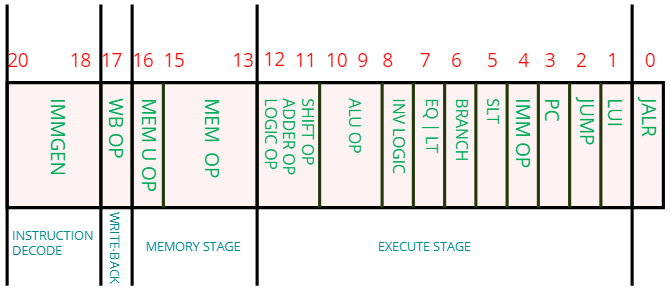
\includegraphics[width=0.7\textwidth]{ControlWord}
			\caption{Control Word Format}
			\label{Image3.3}
		\end{center}
	\end{figure}	

	\vspace{2mm}
	
	Depicted with blue color at Figure \ref{Image3.3} are four groups of bits. These are the bits that concern each pipeline stage. The bit $0$ is used also at ID stage along with bits $20..18$ but it is appended later as Figure \ref{Image3.2} shows and is not hard-type in every input of the multiplexers like the rest of the control signal bits. It is also used for pipeline control.
	
	\clearpage
	\small
	\begin{itemize}
		%\setlength\itemsep{-0.1em}
		\item \textbf{IMMGEN} : Immediate Genaration
		\begin{itemize}
			\setlength\itemsep{-0.1em}
			\item $000$ : I-type Immediate,
			\item $001$ : S-type Immediate.
			\item $010$ : B-type Immediate.
			\item $011$ : U-type Immediate.
			\item $100$ : J-type Immediate.
		\end{itemize}
		\item \textbf{WB OP} : Write Back operation. $0$ if the command doesn't require a Write Back action, $1$ if it does.
		\item \textbf{MEM U OP} : Memory Unsigned Operation. $0\rightarrow NO$, $1\rightarrow YES$.
		\item \textbf{MEM OP} : Memory Operation.
		\begin{itemize}
			\setlength\itemsep{-0.1em}
			\item $000$ : LB 
			\item $001$ : LH
			\item $010$ : LW
			\item $100$ : SB
			\item $101$ : SH
			\item $110$ : SW
			\item $111$ : MEM-Free operation.
		\end{itemize}
		\item \textbf{ALU OP}: ALU Operation 
		\begin{itemize}
			\setlength\itemsep{-0.1em}
			\item $00$ : Addition.
			\item $01$ : Subtraction.
			\item $10$ : Logic Operation.
			\item $11$ : Shift Operation.
		\end{itemize}
		\item \textbf{SHIFT/ADDER/LOGIC OP}: Since bits $[9..8]$ determine which ALU module will be used there is no problem using the same bits $[11..10]$ to represent different operations in different ALU modules. 
		\begin{itemize}
			\setlength\itemsep{-0.3em}
			\item Shift Module:
			\begin{itemize}
				\setlength\itemsep{-0.1em}
				\item $00$ : Shift Right Logical.
				\item $01$ : Shift Left Logical.
				\item $10$ : Shift Right Arithmetic.
			\end{itemize}
			\item Adder Module:
			\begin{itemize}
				\setlength\itemsep{-0.1em}				
				\item $0X$ : Signed Addition or Subtraction.
				\item $1X$ : Unsigned Addition or Subtraction.

			\end{itemize}
			\item Logic Module:
			\begin{itemize}
				\setlength\itemsep{-0.1em}
				\item $00$ : And.
				\item $01$ : Or.
				\item $10$ : Xor.			
			\end{itemize}
		\end{itemize}
		
		\item \textbf{INV}\textbf{ \& EQ/LT}: Used for resolving a branch case. 
		\item \textbf{BRANCH}: $0\rightarrow$ the command is not a Branch, $1\rightarrow$ the command is a Branch.
		\item \textbf{SLT}: $0\rightarrow$ the command is not SLT, $1\rightarrow$ the command is SLT.
		\item \textbf{PC}: $0\rightarrow$ PC is not required for calculations. $1\rightarrow$ PC is required for calculations.
		\item \textbf{JUMP}: $0\rightarrow$ the command is not a JUMP. $1\rightarrow$ command is a JUMP.
		\item \textbf{LUI}: $0\rightarrow$ the command is not a LUI. $1\rightarrow$ the command is a LUI.
		\item \textbf{JALR}: $0\rightarrow$ the command is not a JALR. $1\rightarrow$ the command is a JALR.
	\end{itemize}
	
	\clearpage
		
	\begin{center}
		\begin{threeparttable}[!ht]
			\begin{tabular}{|c|c|} \hline
				
				\setrow{\bfseries}Command &\setrow{\bfseries}Control Word\\\hline
				LB   &000-1-0-000-0X-00-X-X-0-0-1-0-0-0-0 \\\hline
				LH   &000-1-0-001-0X-00-X-X-0-0-1-0-0-0-0\\\hline
				LW   &000-1-0-010-0X-00-X-X-0-0-1-0-0-0-0\\\hline
				LBU  &000-1-1-000-0X-00-X-X-0-0-1-0-0-0-0\\\hline
				LHU  &000-1-1-001-00-00-X-X-0-0-1-0-0-0-0\\\Xhline{5\arrayrulewidth}
				
				ADDI &000-1-X-111-0X-00-X-X-0-0-1-0-0-0-0\\\hline
				SLLI &000-1-X-111-01-11-X-X-0-0-1-0-0-0-0\\\hline
				SLTI &000-1-X-111-0X-01-X-X-0-1-1-0-0-0-0\\\hline 
				SLTIU&000-1-X-111-1X-01-X-X-0-1-1-0-0-0-0\\\hline 
				XORI &000-1-X-111-10-10-X-X-0-0-1-0-0-0-0\\\hline 
				SRLI &000-1-X-111-00-11-X-X-0-0-1-0-0-0-0\\\hline
				SRAI &000-1-X-111-10-11-X-X-0-0-1-0-0-0-0\\\hline
				ORI  &000-1-X-111-01-10-X-X-0-0-1-0-0-0-0\\\hline
				ANDI &000-1-X-111-00-10-X-X-0-0-1-0-0-0-0\\\Xhline{5\arrayrulewidth}
				
				SB &001-0-0-100-0X-00-X-X-0-0-1-0-0-0-0\\\hline
				SH &001-0-0-101-0X-00-X-X-0-0-1-0-0-0-0\\\hline
				SW &001-0-0-110-0X-00-X-X-0-0-1-0-0-0-0\\\Xhline{5\arrayrulewidth}
				
				ADD &XXX-1-X-111-0X-00-0-0-0-0-0-0-0-0-0\\\hline
				SUB &XXX-1-X-111-0X-01-0-0-0-0-0-0-0-0-0\\\hline
				SLL &XXX-1-X-111-01-11-0-0-0-0-0-0-0-0-0\\\hline
				SLT &XXX-1-X-111-0X-01-0-0-0-1-0-0-0-0-0\\\hline
				SLTU&XXX-1-X-111-1X-01-0-0-0-1-0-0-0-0-0\\\hline
				XOR &XXX-1-X-111-10-10-0-0-0-0-0-0-0-0-0\\\hline
				SRL &XXX-1-X-111-00-11-0-0-0-0-0-0-0-0-0\\\hline
				SRA &XXX-1-X-111-10-11-0-0-0-0-0-0-0-0-0\\\hline
				OR  &XXX-1-X-111-01-10-0-0-0-0-0-0-0-0-0\\\hline
				AND &XXX-1-X-111-00-10-0-0-0-0-0-0-0-0-0\\\Xhline{5\arrayrulewidth}
				
				BEQ &010-0-X-111-0X-01-0-1-1-0-0-0-0-0-0\\\hline
				BNE &010-0-X-111-0X-01-1-1-1-0-0-0-0-0-0\\\hline
				BLT &010-0-X-111-0X-01-0-0-1-0-0-0-0-0-0\\\hline
				BGE &010-0-X-111-0X-01-1-0-1-0-0-0-0-0-0\\\hline
				BLTU&010-0-X-111-1X-01-0-0-1-0-0-0-0-0-0\\\hline
				BGEU&010-0-X-111-1X-01-1-0-1-0-0-0-0-0-0\\\Xhline{5\arrayrulewidth}
				
				AUIPC&011-1-X-111-0X-00-X-X-0-0-1-1-0-0-0\\\hline
				LUI  &011-1-X-111-XX-00-X-X-0-0-1-1-0-1-0\\\hline
				JALR &000-1-X-111-01-00-X-X-0-0-1-0-1-0-1\\\hline
				JAL  &100-1-X-111-0X-00-X-X-0-0-1-1-1-0-0\\\Xhline{5\arrayrulewidth}
										
			\end{tabular}
				\begin{tablenotes}
				\footnotesize
				\item 
				Notes:
				\item 	
				"X" stands for "Don't Care". It could be either 1 or 0.
				\end{tablenotes}
				
			 	\captionof{table}{Commands and their Control-Words}
				\label{Table3.2}
				\vspace{3mm}
		\end{threeparttable}
	
\end{center}

	This encoding, is the result of many iterations due to the fact that while being in the second pipeline stage ($ID$) we had to think about what will be needed to be done in the next pipeline stages. Finally, with respect to the encoding, we present the control-words (multiplexer inputs) for every instruction in our ISA.\\

\subsection{\textcolor{orange}{Register File}}
\label{SubSec3.2.3:REG FILE}
	The register file consists of $32$ registers which are $32$-bit wide as our architecture dictates. They all have the function of \textbf{read} and \textbf{write}(parallel load) except for one, the register $0$ which has the value $0$ hardwired inside it. This value cannot be altered meaning the register cannot do a parallel load operation. All other registers have a $RESET$ and a $LOAD$ control signal also which are activated only when a global\footnote{When the CPU starts running, we assume that there will be a short reset to initialize all the pipeline components} reset happens.\\
	
	As shown in Figure \ref{Image3.2} the register file is between a $5\rightarrow32$ decoder and two $32\rightarrow1$ multiplexers.
	The decoder is used for the $WRITE$ operations and the multiplexers are used for the $READ$ operations. Almost every command in our ISA has $5$ bits ($[11..7]$)\footnotemark dedicated for the register $rd$ which is the destination register, meaning the register in whom the result of the command will be written into. In our pipeline architecture this happens at the fifth (Write Back) stage. So, when a command reaches the Write Back stage and if it is a command that has to write a result into a register, then the Write Back provides the $rd$'s address back to the register file along with the value that has to be written (operation's result). The $rd$'s address is connected to the decoder and then the proper $LOAD$ signal is activated so that the register that translates to $rd$'s address will be ready for a $WRITE$ operation.\\
	
	The two multiplexers, are used to provide the operands, $rs1$ and $rs2$ (if any) values for the Execute Stage. They first multiplexer provides the $rs1$ value by using the word's bits$[19..15]$\footnotemark[\value{footnote}]. as selector while the second multiplexer provides the $rs2$ value by using the word's bit$[24..20]$\footnotemark[\value{footnote}]. as selector. Every multiplexer input is paired with every register's output. For example, $Reg_0\rightarrow I_0$, $Reg_1 \rightarrow I_1$, $Reg_2 \rightarrow I_2$ etc. \\
	
	Of course, not every command requires a $rs1$ or $rs2$ value. In this case the register file will provide two values that will be random and that will not be needed. Later, we add further logic components to resolve this issue. 
	
	
	\footnotetext{You can refer to Figure \ref{Image2.2} for any clarifications needed.}
	
\vspace{5mm}
\subsection{\textcolor{burgundy}{Immediate Generator}}
\label{SubSec3.2.4:IMMGEN}
The Immediate Genarator module is responsible for providining the immediate that is required according to the instruction that is being decoded. It uses the three bits$[20..18]$of the control word(Figure \ref{Image3.3})  and according to them, formats the proper immediate as Figure \ref{Image2.3} shows; by rearranging and manipulating the bits of the fetched word. When this procedure is over, the bits$[20.18]$ of the control word are no longer needed and thus they are removed of the control-word, before it leaves the $ID$ stage. The immediate generator module implements the following algorithm;

\clearpage

\begin{algorithm}[H]
	\SetAlgoLined
	\SetKwInOut{Input}{input}\SetKwInOut{Output}{output}
	
	\Input{ $CONTROL\_WORD[20..18]$ and $FETCHED\_WORD$}
	\Output{$IMMEDIATE$} 
	\BlankLine
	
	\emph{IMM\_TYPE $\leftarrow$ CONTROL\_WORD[20..18]}\;
	\uIf	{IMM\_TYPE == "000"} { {\small $IMMEDIATE$ =  \underline{I-type} Immediate, f(\footnotesize{$FETCHED\_WORD$})} \;}
	\uElseIf{IMM\_TYPE == "001"} { {\small $IMMEDIATE$ =  \underline{S-type} Immediate, f(\footnotesize{$FETCHED\_WORD$})} \;}
	\uElseIf{IMM\_TYPE == "010"} { {\small $IMMEDIATE$ =  \underline{B-type} Immediate, f(\footnotesize{$FETCHED\_WORD$})} \;}
	\uElseIf{IMM\_TYPE == "011"} { {\small $IMMEDIATE$ =  \underline{U-type} Immediate, f(\footnotesize{$FETCHED\_WORD$})} \;}
	\uElseIf{IMM\_TYPE == "100"} { {\small $IMMEDIATE$ =  \underline{J-type} Immediate, f(\footnotesize{$FETCHED\_WORD$})} \;}
	\Else{ {\small $IMMEDIATE$ =  \underline{XXX..X}} \;}
	
	\caption{Immediate Generator Algorithm}
	\label{Algorithm1}
\end{algorithm}	
\vspace{5mm}

\subsection{\textcolor{byzantium}{Adder}}
\label{SubSec3.2.5:ADDER}

In the the case of Uncoditional Jumps, two calculations are required. The calculation of the target address, and the storing of the next instruction's address, the return address,($PC+4$) to register rd. This translates into two addition operations that must be done in the event of those commands. All the computational force in a pipeline usually is entrusted to the pipeline's ALU\footnote{Arithmetic and Logic Unit}. In our pipeline ALU lays in the third stage, the $Execute$ stage. So we would have to equip the ALU module with two Adders since when a jump is imminent, two additions should be done. To relieve some workload of the ALU's design we decided to equip the $ID$ module with one of those two adders, an adder that will be responsible only for the calculation of the target address of the unconditional jumps. \\

In theory, this would work fine, since all the necessary operands are available at $ID$ stage. After further investigating the $JALR$ command though, we see that the target address is calculated in a different way. Instead of $PC+IMM$, $JALR$ dictates that the target address is calculated as $PC+RS1$. So this means that first, we have to access the register file to acquire the one of the two operands and then do the addition operation, since the $PC$ value is already available (from the $IF$ stage). In practice, we found that due to some propagation delays we should handle the $JALR$ case differently. \\ 
\clearpage
What we did to resolve this, is to treat the $JAL$ and $JALR$ commands in $ID$ like this:

\begin{itemize}
	\setlength\itemsep{-0.1em}
	\item If the command is $JAL$ then:
		\begin{itemize}
			\item Calculate the $TARGET\_ADDRESS$ as $PC+IMMEDIATE$.
		\end{itemize}
	\item If the command is $JALR$ then:
		\begin{itemize}
			\item Calculate the $RETURN\_ADRESS$ as $PC+4$.
		\end{itemize}
\end{itemize}

\vspace{2mm}

This is achieved by adding a $2\rightarrow1$ multiplexer that selects by $CONTROL\_WORD[0]$ - ($JALR$) either the $IMMEDIATE$ or the constant $+4$. So for $JAL$ we leave the calculation of the jump's return address to the $Execute$ stage and for $JALR$ we leave the calculation of the jump's target address to the $Execute$ stage.

\subsection{\textcolor{ao}{Stall \& Forward Predictor}}
\label{SubSec3.2.6:STALLFWD}
This is a module that was added later on $ID$ and it is responsible for detecting whether a stall or a forwarding is required. Forwarding (or Bypassing) is the counter-measure of the true dependency RAW\footnote{Read After Write}, which is the only threat in our system, since we do not support OOO\footnote{Out Of Order execution}.

\begin{figure}[h!]
	\begin{center}
		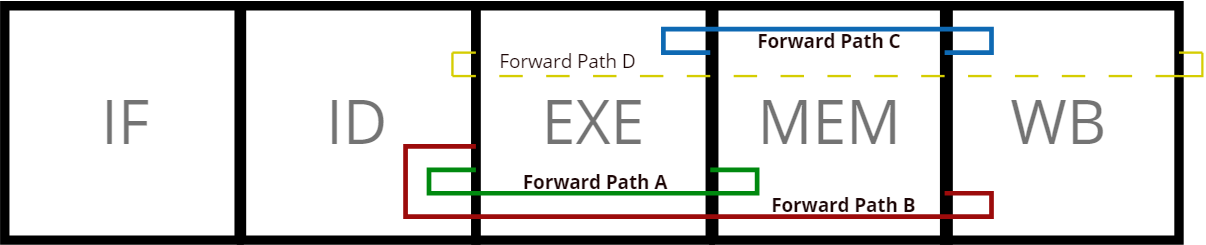
\includegraphics[width=1\textwidth]{FORWARDS}
		\caption{Forwarding Paths}
		\label{Image3.4}
	\end{center}
\end{figure}
\vspace{2mm}

The module is responsible for handling Forwards A,B, and C, while forward D\footnote{We will analyze the Forward D later.} is being handled by some external logic. So there are three main RAW scenarios that require resolution.

\subsubsection{Scenario A} 
\label{3.2.6.1}

\begin{lstlisting}[caption={Forward Path A Example},captionpos=b]
	OP_A	Reg_X, Reg_A, Reg_B
	OP_B 	Reg_Y, Reg_X, Reg_C
\end{lstlisting}



This scenario concerns the $ID$ and $Execute$ stages. OP\_A writes its result to Reg\_X. Then OP\_B requires Reg\_X's value as $rs1$ operand. Without the forwarding path, we would have to stall for at least two clock cycles and wait for OP\_A to reach the $Write\ Back$ stage. We know that the value that will be written at at Reg\_X will be available at the end of $Execute$ stage. So instead of stalling for two clock cycles, we activate the Forward Path A and transfer the value needed to OP\_B.

\clearpage

\subsubsection{Scenario B}
\label{3.2.6.2}

\begin{lstlisting}[caption={Forward Path B Example},captionpos=b]
	OP_A	Reg_X, Reg_A, Reg_B
	....	.....  .....  .....
	OP_B 	Reg_Y, Reg_X, Reg_C
\end{lstlisting}

This scenario concerns the $ID$ and $Memory$ stages. Once again OP\_A writes its result to Reg\_X and then, after one command that is in-between them, OP\_B requires this value as an operand. If not for the Forward Path B, we would have to stall again for one clock cycle and wait for OP\_A to reach the $Write\ Back$ stage.

\subsubsection{Scenario C}
\label{3.2.6.3}

\begin{lstlisting}[caption={Forward Path C Example},captionpos=b]
	LOAD 	Reg_X, IMM(Reg_A)
	STORE	Reg_X, IMM(Reg_B)
\end{lstlisting}

This scenario concerns only the $Memory$ stage. It only occurs when there is a $STORE$ command after a $LOAD$ command, of whom the later wishes to write in the memory the register value that the first has loaded. We would normally have to stall for one clock cycle again but with the Forward Path C we can overcome this issue. 

\subsubsection{Stall Generation}
\label{3.2.6.4}
\begin{lstlisting}[caption={Stall Scenario},captionpos=b]
	LOAD 	Reg_X, IMM(Reg_A)
	OP_A	Reg_A, Reg_X, Reg_B
\end{lstlisting}

In this case, we have to stall the OP\_A and those who follow, because the $LOAD$ command, has to reach the $Memory$ stage and then, activate the Forward Path B so that it can provide the needed value. This happens due to the nature of the $LOAD$ commands, which have their result ready at the end of $Memory$ stage and not at the $Execute$ stage like the other computational commands.\\

\footnotesize
\begin{algorithm}[H]
	\SetAlgoLined
	\SetKwInOut{Input}{input}\SetKwInOut{Output}{output}
	
	\Input{ $RS1[4..0]$,$RS2[4..0]$, $RD\_IN\_EXE[4..0]$, $RD\_IN\_MEMORY[4..0]$, $LOAD\_IN\_EXE$, $CONTROL_WORD[20..18]$}
	\Output{ $FWDA[2]$, $FWDB[2]$, $FWDC$, $STALL$} 
	\BlankLine
	\BlankLine
	\BlankLine
	/* Initialization */ \\
	\emph{ $FWDA[2]\ = \ \{0,0\}$}\;
	\emph{ $FWDB[2]\ = \ \{0,0\}$}\;
	\emph{ $FWDC\ = \ 0$}\;
	\emph{ $STALL\ = \ 0$} \;
	\BlankLine
	\BlankLine
	/* Identify the Type of the Command in ID  */ \\
	\emph{ $COMMAND\_IN\_ID \leftarrow f({\scriptsize CONTROL\_WORD[20..18]})$ {\footnotesize= (R/S/U/B/J)}} \;
	\BlankLine
	\BlankLine
	/* Equality Check between RS1,RS2 and RD in EXE and MEM */\\
	\If{ $RS1$ == $RD\_IN\_EXE$ AND \underline{$RS1\neq REG_{0}$}} {  $FWD\_A\_RS1 \leftarrow 1$\;}
	\If{ $RS2$ == $RD\_IN\_EXE$ AND \underline{$RS2\neq REG_{0}$}} {  $FWD\_A\_RS2 \leftarrow 1$\;}
	\If{ $RS1$ == $RD\_IN\_MEM$ AND \underline{$RS1\neq REG_{0}$}} {  $FWD\_B\_RS1 \leftarrow 1$\;}
	\If{ $RS2$ == $RD\_IN\_MEM$ AND \underline{$RS2\neq REG_{0}$}} {  $FWD\_B\_RS2 \leftarrow 1$\;}
	\BlankLine
	\BlankLine
	/* Check if the command in ID has an RS1 , RS2 register on its type */ \\
	\eIf{ $COMMAND\_IN\_ID \neq U/J-type$ \footnote{If the Command in $ID$ is of U or J type then it does not have an $rs1$ register, hence we must not activate a forward signal}} 
	{ $FWDA[0] \ = \ FWD\_A\_RS1;$ \\ $FWDB[0] \ = \ FWD\_B\_RS1;$}
	{ $FWDA[0] \ = \ 0;$ \\ $FWDB[0] \ = \ 0;$ }
	
	\eIf{ $COMMAND\_IN\_ID = S/B/R-type$  \footnote{Only the Stores, Branches and R-type commands have an $rs2$ register and so, a forward signal for $rs2$ is required only in their case}} 
	{ $FWDA[1] \ = \ FWD\_A\_RS2;$ \\ $FWDB[1] \ = \ FWD\_B\_RS2;$ }
	{ $FWDA[1] \ = \ 0;$ \\ $FWDB[1] \ = \ 0;$ }
	
	\If{$LOAD\_IN\_EXE = 1$ AND $COMMAND\_IN\_ID = S-type$}
	{ $FWDC \ = \ 1;$}
	
	\If{ $LOAD\_IN\_EXE = 1$ AND $(FWD\_A\_RS1$ OR $FWD\_A\_RS2)$}
	{ $STALL \ = \ 1;$}
	
	\caption{Stall and Forward Predictor Algorithm}
	\label{Algorithm2}
\end{algorithm}	

\clearpage

\section{Execute Stage - EXE}
\label{Sec3.3:EXE}
	\small
	The $Execute$, is the third stage in our pipeline. This is where all the computational force of our system is located. It consists by three main parts. The Adder/Subtractor, the Barrel Shifter and the Logical Module. Furthermore, this is the stage in which we decide whether to follow a Branch or not. 
	 
	\begin{figure}[h!]
		\begin{center}
			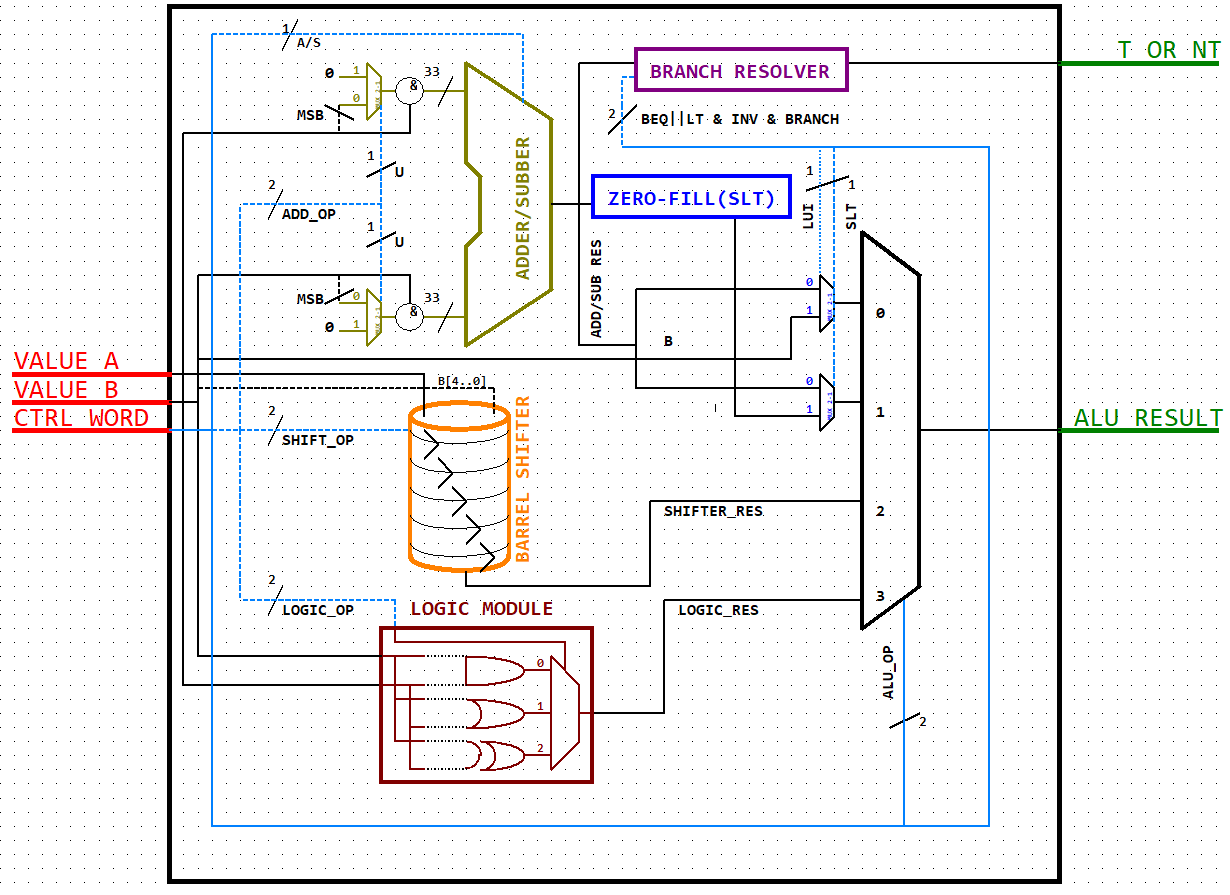
\includegraphics[width=1\textwidth]{EXE}
			\caption{Execute Stage schematic}
			\label{Image3.5}
		\end{center}
	\end{figure}
	
	\vspace{-8mm}
	\subsection{Module's I/O}
	\label{SubSec3.3.1:I/O}
	
		 {\small
		\renewcommand{\labelenumii}{\Roman{enumii}}
		\begin{itemize}
			\item Inputs:
			\begin{enumerate}
				
				\item \textcolor{red}{$VALUE\_A$}      : The first of two operands (32-bits).
				\item \textcolor{red}{$VALUE\_B$} 	  : The second operand (32-bits).
				\item \textcolor{red}{$CTRL\_WORD$}    : Control Signals from $ID$ (9-bits). 
				\begin{itemize}
					\setlength\itemsep{+0.1em}
					{\scriptsize
					\item\textbf{bits[8..7]:} ADD\_OP/SHIFT\_OP/LOGIC\_OP. 
					\item\textbf{bits[6..5]:} ALU\_OP.
					\item\textbf{bit[3]:} EQ/LT.
					\item\textbf{bit[2]:} BRANCH. 
					\item\textbf{bit[1]:} SLT. 
					\item\textbf{bit[0]:} LUI.
					
				    }
				\end{itemize}
			\end{enumerate}
			\item Outputs:
			\begin{enumerate}
				
				\item \textcolor{forestgreen(web)}{$T\_OR\_NT$} : Branch condition result (1-bit).
				\item \textcolor{forestgreen(web)}{$ALU\_RES$} : (32-bit).
			\end{enumerate}
	\end{itemize}}
	\vspace{5mm}
	
	\clearpage
	\small
	Note that we only use 9 out of the total 18 control bits which were generated by the $ID$ stage. This happens because we simply do not have any use for the other bits, hence we use a logic - circuit between the pipeline registers  to separate them respectively, meaning the pipeline stage that they must be addressed to, and then in every clock cycle distribute them to the designated location.
	
	\subsection{\textcolor{olive}{Adder / Subtractor}}
	\label{SubSec3.3.2:ADD/SUB}
	This module is responsible for doing Signed and Unsigned addition and subtraction. It is in its core a ripple-carry architecture in which we added a few customizations on our own. Besides the typical modulation the circuit requires so it can do a subtraction (2's complement on B operand) as one can notice in Figure \ref{Image3.5} the module's inputs have a $2\rightarrow1$ multiplexer controlled by the select bit$[8]$ which in case of addition or subtraction stands for Signed/Unsigned operation. \\
	
	Normally as mentioned before, we do not care for Overflow scenarios and we leave this to the programmer's hands. But there is a case that an overflow could be disastrous for us, an overflow in signed subtraction operations. If two numbers are subtracted and their signs are different, then overflow occurs if and only if the result has the same sign as the subtrahend\footnote{What is being subtracted.}. For example, lets say we have a module that subtracts 3-bit numbers. In this module we insert as minuend\footnote{What is being subtracted from.} 
	the number $011 (+3)$ and as subtrahend the number $101 (-3)$. 
	
	\begin{figure}[h!]
		\begin{center}
			\fbox{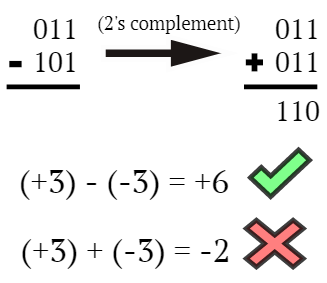
\includegraphics[width=0.4\textwidth]{SUB_OVERFLOW}}
			\caption{Overflow example}
			\label{Image3.6}
		\end{center}
	\end{figure}
	\vspace{-4mm}
	
	This problem should not bother us since we leave this issue to the programmer, but in some cases like the case of an unconditional jump command, this fault could be catastrophic. In order to evaluate if we must take or not the jump, we do a subtraction and then check for the difference's sign to decide. The problem mentioned above would make us pick mistakenly the wrong path and loose the branch.\\
	
	Since the sign is the most important information that we might loose with the overflow issue, we could overcome this by adding one extra bit to our operands. Instead of subtracting 32-bit numbers we could sign-extend the values up to 33-bits and then continuing with the operation without any risks of sign alteration at the results. With the same numbers as operands, we attach this logic to the previous example.
	
	\begin{figure}[h!]
		\begin{center}
			\fbox{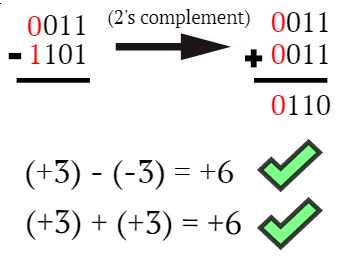
\includegraphics[width=0.4\textwidth]{SUB_OVERFLOW_SOLVED}}
			\caption{Overflow prohibit example}
			\label{Image3.7}
		\end{center}
	\end{figure}
	\vspace{-4mm}
	
	With respect to the logic that was analyzed above, we use a 33-bit Adder/Subtractor in our ALU that does Signed operations by 
	using sign-extension up to 33-bits and Unsigned operations by using zero-fill up to 33-bits. Since we add 1 extra bit to our module for signed actions we have to utilize it properly for the unsigned ones. Hence, we use zero-fill instead for all the Unsigned operations so that the result will not be corrupted. The two $2\rightarrow1$ multiplexers are responsible for the sign-extension/zero-fill and then the selected value is concatenated to the operands' MSB\footnote{Most Significant Bit.} \\ 
	
	Since our architecture is 32-bit, we cannot simply continue with 33-bit values in our pipeline. The result of the Adder/Subtractor gets cropped down to 32-bits while the 33rd bit is being used by other modules (e.g $BRANCH\_RESOLVER$) for further computations. 
	
	\begin{figure}[h!]
		\begin{center}
			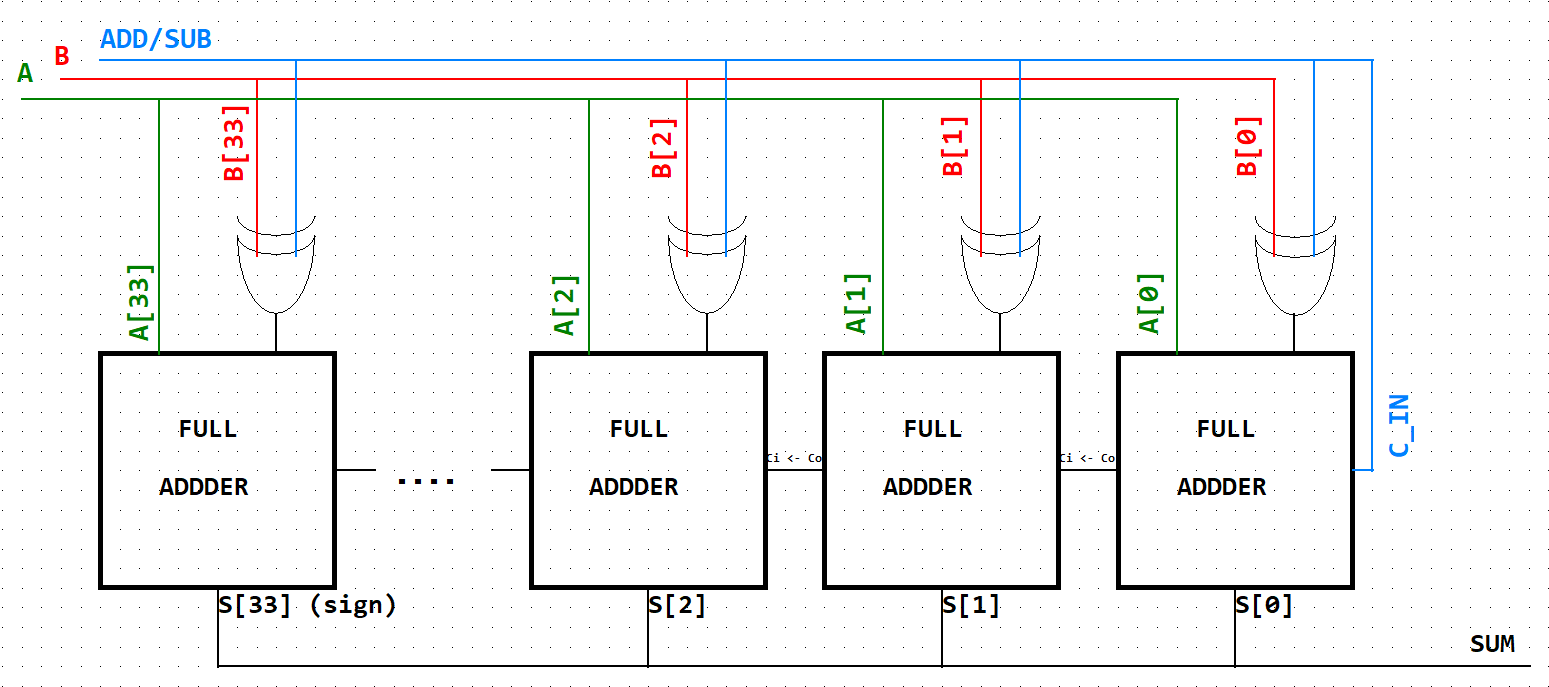
\includegraphics[width=1\textwidth]{RIPPLE_ADDER}
			\caption{Adder/Subtractor module}
			\label{Image3.8}
		\end{center}
	\end{figure}
	
	\subsubsection{Commands that Use The Module}

	With respect to the sequential order that the Table \ref{Table 3.1} declares, here is a list of the commands that utilize the Adder/Subtractor module.
	
	\vspace{2mm}
	\begin{threeparttable}[h!]
		
		\begin{tabular}{|l|l|c|} \hline
				\setrow{\bfseries}Command  &\setrow{\bfseries} Reason &\setrow{\bfseries} Comment \\\hline
				AUIPC    & $IMMEDIATE\ +\ PC$  & -\\\hline
				JAL   	 & $PC\ + \ 4 $  	   & {\footnotesize Next command's address }\\\hline
				JALR  	 & $PC\ + \ RS1$	   & {\footnotesize Target address } \\\hline 
				BRANCHES & $RS1\ - \ RS2$ 	   & {\footnotesize Equality/Inequality check }\\\hline
				LOADS 	 & $RS1\ + \ IMMEDIATE$& {\footnotesize Effective address}\\\hline
				STORES   & $RS1\ + \ IMMEDIATE$& {\footnotesize Effective address}\\\hline
				ADDI	 & $RS1\ + \ IMMEDIATE$& -\\\hline
				SLTI[U]  & $RS1\ - \ IMMEDIATE$& {\footnotesize The sign of the result will be the value for $rd$\footnotemark} \\\hline	 
				ADD 	 & $RS1\ + \ RS2$	   & -\\\hline
				SUB	 	 & $RS1\ - \ RS2$	   & -\\\hline
				SLT[U]	 & $RS1\ - \ RS2$	   & Same as SLTI[U] \\\hline
		\end{tabular}
		
		\captionof{table}{Commands that use the Adder/Subtractor}
		\label{Table 3.3}
		\vspace{5mm}
	\end{threeparttable}

	\footnotetext{If $RS1 - IMMEDIATE < 0$ then the result will have bit$[33]$ (sign) = 1. So we can easily handle this command by only looking the result's sign }
	
	\subsection{\textcolor{orange}{Barrel Shifter}}
	\label{SubSec3.3.3:BARREL}
	
	The barrel shifter is a digital circuit that can shift a data word by a specified number of bits \footnote{Shift amount (shamt).} in just \underline{1 clock cycle} without the use of any sequential logic, only pure combinatorial logic. The way we implemented it is as a sequence of multiplexers where the output of one multiplexer is connected to the input of the next multiplexer in a way that depends on the \textbf{shift distance}. Generally the number of multiplexers required for an n-bit word is $nlog_{2}(n)$; in our case we have 32-bit words hence normally we would need $32log_{2}(32) = 160$ multiplexers in total. \\
	
	Our system has 32-bit words, which can be shifted up to 32 slots left or right. So to represent the shift amount (shamt) we need $log_2(32) = 5$ bits. According to those five bits we separate the shifting operation into stages:

	\begin{itemize}
		\setlength\itemsep{-0.1em}
		\item \textbf{Stage \#1:} Shift by 16; controlled by shamt[4].
		\item \textbf{Stage \#2:} Shift by 8 ; controlled by shamt[3].
		\item \textbf{Stage \#3:} Shift by 4 ; controlled by shamt[2].
		\item \textbf{Stage \#4:} Shift by 2 ; controlled by shamt[1].
		\item \textbf{Stage \#5:} Shift by 1 ; controlled by shamt[0].
	\end{itemize}

	In every shifting stage we need multiplexers to represent each bit of the data word which is being shifted, so every stage needs 32 multiplexers. This is how the number $160$ comes up. But, our barrel shifter module must be able to do, right arithmetic, right, and left shifting operations. We need $160$ multiplexers for just right or left shift. To be able to do all three kinds of shift we have to use more circuitry; in fact we used $[2 \times 32log_{2}(32)] + 1 = 321$ multiplexers:
	
	\begin{itemize}
		\setlength\itemsep{-0.1em}
		\item For each stage we use two multiplexers instead of one ( $\mathbf{2\times}$ ).
		\item We have five stages for every bit of the shifting word ( $\mathbf{32log_{2}(32)}$ ).
		\item We use one extra multiplexer for right arithmetic shifts ( $\textbf{+1}$ ).
		
	\end{itemize}

	The barrel shifter requires 2 control bits to do one of the shifts. Note the MSB signifies the Arithmetic shift, while the LSB the left or right shift.
	
	\begin{center}
		\begin{tabular}{|c|c|} \hline
			
			\setrow{\bfseries}Shift Type  &\setrow{\bfseries} Control Word \\\hline
			Right			 & 0-0 \\\hline
			Left   			 & 0-1 \\\hline
			Right Arithmetic & 1-0 \\\Xhline{5\arrayrulewidth}
			ERROR 	    	 & 1-1 \\\hline
		\end{tabular}
	\end{center}

	
	\begin{figure}[h!]
		\begin{center}
			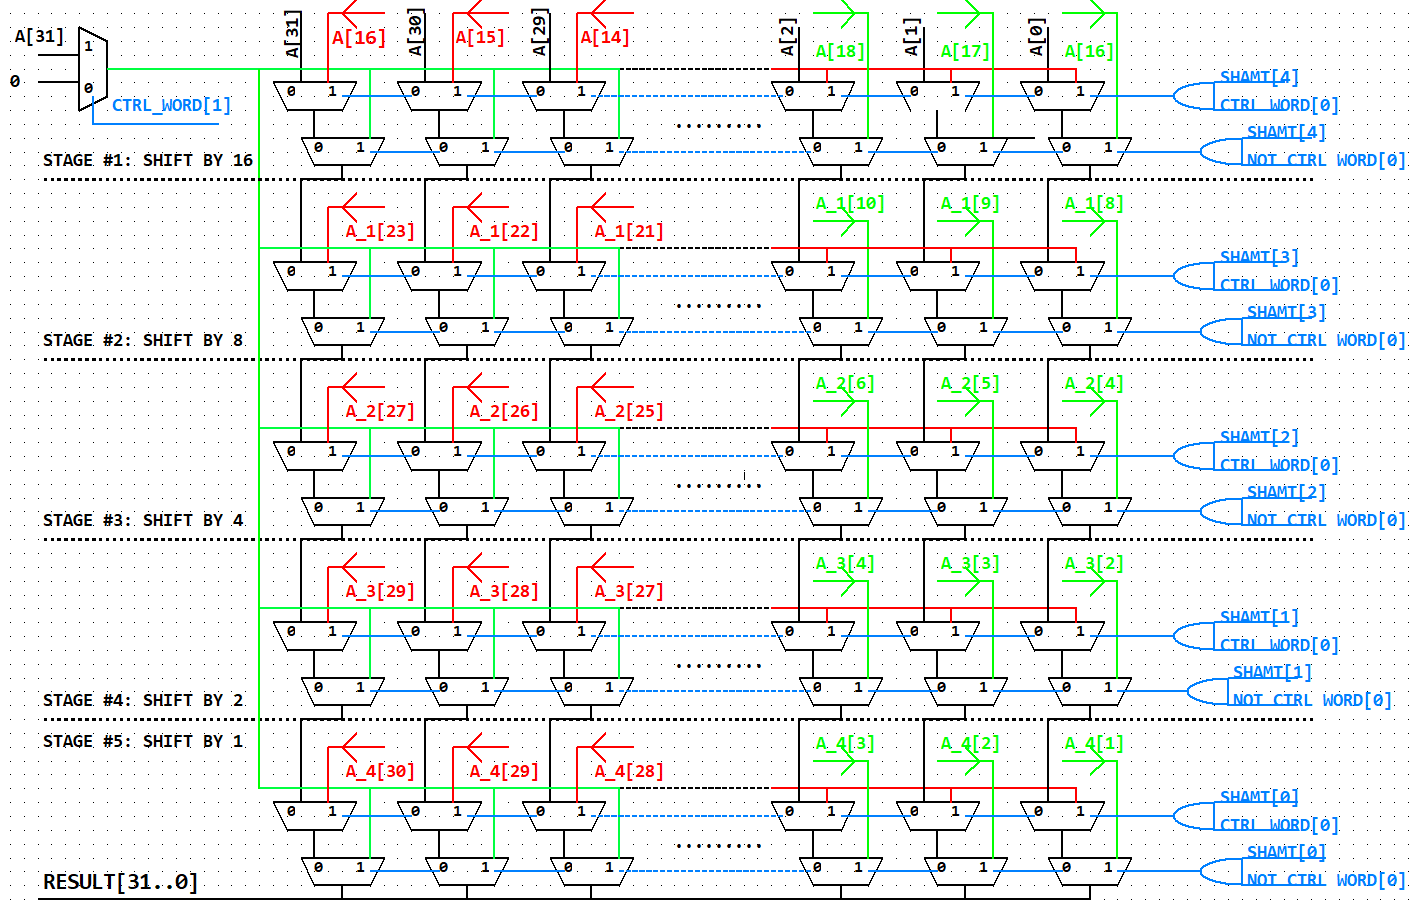
\includegraphics[width = 1\textwidth,height=0.5\textheight]{BARREL_SHIFTER2}
			\caption{Barrel Shifter module.}
			\label{Image3.9}
		\end{center}
	\end{figure}

	All the theory mentioned above is now aggregated into Figure \ref{Image3.9}. There are five shifting stages and for every bit we use two multiplexers where the top one is responsible for handling the left shifts and the bottom one the right and the right arithmetic shifts. 
	
	\clearpage
	
	\subsubsection{Commands that Use The Module}
	
	The commands that utilize the barrel shifter module are the following:
	
	\vspace{2mm}
	\begin{threeparttable}[h!]
		
		\begin{tabular}{|l|l|c|} \hline
			\setrow{\bfseries}Command  &\setrow{\bfseries} Reason &\setrow{\bfseries} Comment \\\hline
			SLLI     & $RS1 << IMM$		    & -\\\hline
			SRLI     & $RS1 >> IMM$		    & -\\\hline
			SRAI     & $RS1 >> IMM$		    & Vacant positions are filled with MSB\\\hline
			SLL      & $RS1 << RS2[5..0]$   & -\\\hline
			SRL      & $RS1 >> RS2[5..0]$   & -\\\hline
			SRA 	 & $RS1 >> RS2[5..0]$   & Vacant positions are filled with MSB\\\hline
			
		\end{tabular}
		
		\captionof{table}{Commands that use the Barrel Shifter}
		\label{Table 3.4}
		\vspace{3mm}
	\end{threeparttable}

	\subsection{\textcolor{burgundy}{Logic Module}}
	\label{SubSec3.3.4:LOG}
	
	The logic module is the simplest part in our ALU. It consists of three large logical gates, the AND, the OR and the XOR, which are $32$-bit wide. The two inputs for each gate are the two operands of the ALU, A and B. The module's output is selected from a $4\rightarrow1$ multiplexer which has two control bits as selector, the bits$[12..11]$ of the control word (Figure \ref{Image3.3}).
	
	 \subsubsection{Commands that Use The Module}
	 
	 The commands that utilize the logic module are the following:
	 
	 \vspace{2mm}
	 \begin{center}
	 \begin{threeparttable}[h!]
	 	
	 	\begin{tabular}{|l|l|c|} \hline
	 		\setrow{\bfseries}Command  &\setrow{\bfseries} Reason &\setrow{\bfseries} Comment \\\hline
	 	    XORI     & $RS1 \oplus IMM$		& -\\\hline
	 		ORI      & $RS1 +  IMM$			& -\\\hline
	 		AND      & $RS1 \land  IMM$		& -\\\hline
	 		XOR      & $RS1 \oplus RS2$		& -\\\hline
	 		OR       & $RS1 +  RS2$     	& -\\\hline
	 		AND 	 & $RS1 \land RS2$      & -\\\hline
	 		
	 	\end{tabular}
	 	
	 	\captionof{table}{{\scriptsize Commands that use the Logic Module}}
	 	\label{Table 3.5}
	 	\vspace{3mm}
	 \end{threeparttable}
 	 \end{center}
  
  	\clearpage
  	
  	\subsection{\textcolor{byzantium} {Branch Resolver}}
  	The Branch Resolver module is responsible for determining whether we should follow or not a Branch Unconditional Jump. Note that our design does not posses a branch prediction unit and so we deal with branch cases in Execute stage. This means, that if the branch is finally $Taken$ that we have to flush the previous two pipeline stages ($IF$,$ID$) because the commands that have been fetched are not valid anymore. \\
  	
  	It takes as input three control bits and the result of the Adder/Subtractor module. It works according to the following truth table:
  	
  	\begin{center}
  		
  		\begin{tabular}{|c|c|c|c|} \hline
  		\setrow{\bfseries}Command &\setrow{\bfseries} BEQ &\setrow{\bfseries} INVERT LOGIC &\ \setrow{\bfseries}BRANCH \\\hline
  		BEQ     & 1 & 0 & 1 \\\hline
  		BNE     & 1 & 1 & 1 \\\hline
  		BLT     & 0 & 0 & 1 \\\hline
  		BGE     & 0 & 1 & 1 \\\hline
	  	\end{tabular}
  
  	 	\captionof{table}{ Branch Command Encoding }
  		\label{Table 3.7}
	
  	\end{center}
  	  	
  	\begin{figure}[h!]
  		\begin{center}
  			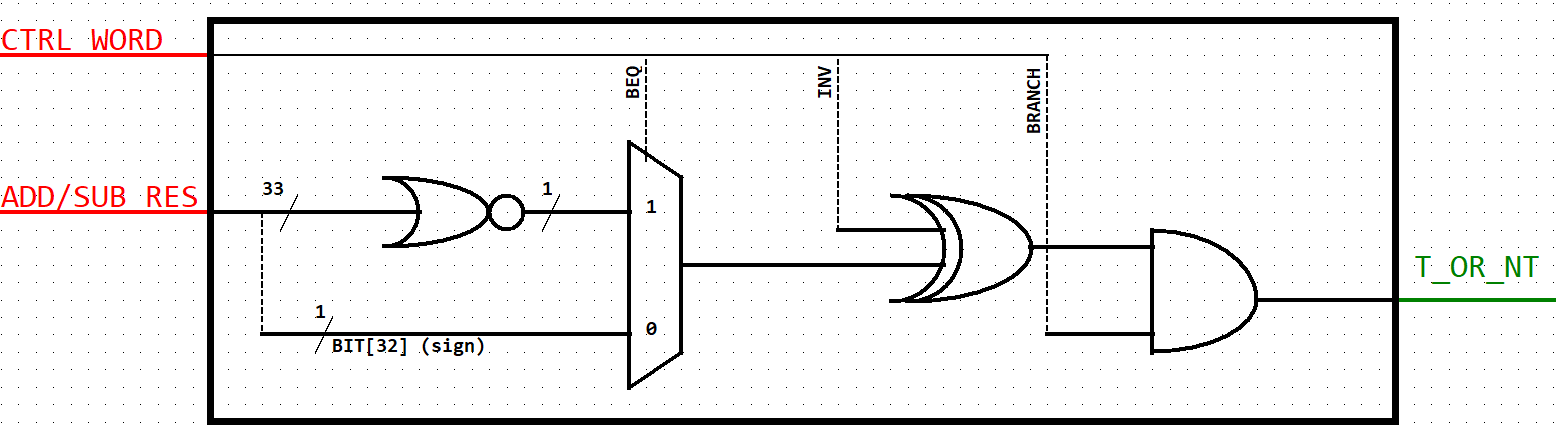
\includegraphics[width=1\textwidth]{EXE_BRANCH_RESOLVE}
  			\caption{Branch Predictor Module}
  			\label{Image3.10}
  		\end{center}
  	\end{figure}
  	
  	\vspace{-4mm}
  	
    The general idea for the development of this module was the following:
    \begin{center}
    	$\mathbf{ A \ relop \ B \Longleftrightarrow A - B < 0}$ \footnote{We can easily check the result (sign - bit) of the subtraction's result}
    \end{center}
    We determine equalities and inequalities via subtraction and then we modulate the result (Adder/Subtractor feed) and decide with the circuit of Figure \ref{Image3.10} if we must Take or Not the jump. Reminder; the result from the $ADD/SUB\_RES$ is 33 bits and not 32, due to the overflow avoidance strategy we chose.
  	\vspace{-1mm}
	\subsection{\textcolor{ao}{SLT Module}}
	\label{SubSec3.3.5:SLT}

  	This module is dedicated purely to the Set Less Than (SLT) command. It is simply takes the sign bit of the Adder/Subtractor module and zero-fills it up to 32-bits. So the output of the module will be either $0$ or $1$, which are the two options for the SLT command result. For example: 
  	\begin{footnotesize}
  		\begin{itemize}
  			\item $SLT\  REG\_X, 1,2\  ::\  1 - 2 = -1$ (bit[33] = 1) so the result is 1.
  			\item $SLT\  REG\_X, 2,1\  ::\  2 - 1 = +1$ (bit[33] = 0) so the result is 0.
  		\end{itemize}
  	\end{footnotesize}
  	
  	\clearpage
  	
  	
  \subsection{ALU Output}
  \label{SubSec3.3.6:ALUOUT}
  
  All the results of the stage's modules, are accumulated to the $4\rightarrow1$ multiplexer (Figure \ref{Image3.5}). The multiplexers inputs are selected according to the control word bits$[10..9]$. Furthermore there are two extra $2\rightarrow1$ multiplexers which are responsible for the LUI, and SLT commands. \\
  
  The Load Upper Immediate (LUI) command, does not require any computational effort from our ALU unit. It simply stores a U-Immediate to the $rd$ register. So, we encoded it accordingly and used the same ALU OPCODE with the Additions. So the first $2\rightarrow1$ multiplexer (with control bit$[1]$ as selector) is responsible for providing this U-Immediate in the case of the LUI commands.\\
  
  In a similar way we used another $2\rightarrow1$ multiplexer (with control bit$[5]$ as selector) for the SLT command, but in this case since the command uses the Adder/Subtractor module to perform a subtraction operation, we used the ALU OPCODE of the Subtraction operations. 
  \clearpage
  
\section{Memory Stage - MEM}
  \label{Sec3.4:MEM}
  
  The fourth stage in our pipeline is the $Memory$ stage. This stage is used exclusively by $LOAD$ and $STORE$ commands. Here lies another M4K memory block which simulates the Data Cache (D\$) of our system. 
  Usually in a modern CPU the D\$ is organized as a hierarchy of more cache levels (L1,L2, etc.) but we used a simple memory block for the needs of our project. Also this is the place where global variables in a piece of code are being stored (.data field). For more information concerning the M4K memory blocks we used (I\$ and D\$), you can read \href{https://www.intel.com/content/dam/www/programmable/us/en/pdfs/literature/an/an207.pdf}{Altera's Internal Memory (RAM and ROM) User Guide} and \href{https://www.intel.com/content/dam/www/programmable/us/en/pdfs/literature/ug/ug_ram_rom.pdf}{Intel's Embedded Memory User Guide}.
  
  \begin{figure}[h!]
  	\begin{center}
  		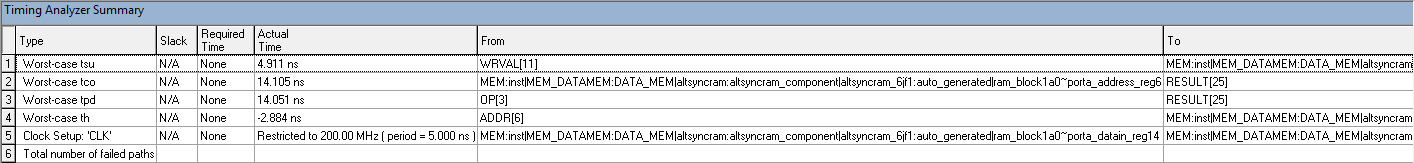
\includegraphics[width=1\textwidth]{MEM}
  		\caption{Memory Stage schematic}
  		\label{Image3.11}
  	\end{center}
  \end{figure}

  \vspace{-5mm}

  The D\$ we used has 128 cells which are 32-bit wide. Hence to iterate through all of them we need $log_{2}(128) = 7$ bits. Those 7 bits are acquired from the result that ALU provides to the pipeline. We isolate from those 32-bits of the result the nine (9) LSBs, of whom the bits$[1..0]$ are used for padding in case of a byte or a half load/store operation. Last but not least the $MEMOP$ control signal \footnote{ Refer to Table \ref{Table3.2} for more information about the command encoding.} is $111$ for the commands that are neither $STORE$ nor $LOAD$ and so we use a reduction NOR gate to generate an $ENABLE$ signal for our D\$ \footnote{Also, MEMOP[2] is used as a Write Enable signal because its 0 for $LOADS$}.
  
  \vspace{-3mm}
  
  \subsection{Module's I/O}
  \label{SubSec3.4.1:I/O}
  
  	\renewcommand{\labelenumii}{\Roman{enumii}}
  \begin{itemize}
  	\item Inputs:
  	\begin{enumerate}
  		\item \textcolor{red}{$CLOCK$} : Global Clock.
  		\item \textcolor{red}{$ALU\_RES$} : LSBs from the ALU to be used as address and padding bits (9-bits).
  		\item \textcolor{red}{$RS2\_VALUE$} : The value that will be written (32-bits) 
  		\item \textcolor{red}{$CTRL\_WORD$} : Control Signals from $ID$ (4-bits). 
  		\begin{itemize}
  			\setlength\itemsep{+0.1em}
  			{\scriptsize
  				\item\textbf{bit[3]:} Signed or Unsigned Load. 
  				\item\textbf{bits[2..0]:} Memory Operation (see \hyperlink{page.18}{page 18 for details}).
  			}
  		\end{itemize}
  	
  	\end{enumerate}
  	\item Outputs:
  	\begin{enumerate}
  		
  		\item \textcolor{forestgreen(web)}{$LOADED\_WORD$} : Word read from D\$ (32-bits).
  	\end{enumerate}
\end{itemize}

\clearpage

\subsection{\textcolor{olive}{Byte Enable Module}}
\label{SubSec3.4.2:BYTEEN}

The M4K Memory block, allows the user to write also in specific bytes inside a memory cell ($BYTEEN$). In our case since we have 32-bit cells we can divide the memory cell into four blocks and alternate each one of them conveniently with our system's SB (Store Byte) command. Furthermore we can modify two bytes inside a memory cell. This means that we can write either on bits$[31..16]$ or bits$[15..0]$ of a memory cell with the SH (Store Half) command.\\ 

To achieve that, we must also have a number that will imply the byte or the bytes that will be written inside the memory cell. With respect to everything mentioned above, we use the two LSBs of the address ($ALU\_RES$) value as an iterator for every memory cell. For referring to a byte half we use the bit$[1]$ of the $ALU\_RES$ and for bytes we use the bits$[1..0]$ as Figure \ref{Image3.12} depicts.

\begin{figure}[h!]
	\begin{center}
		\fbox{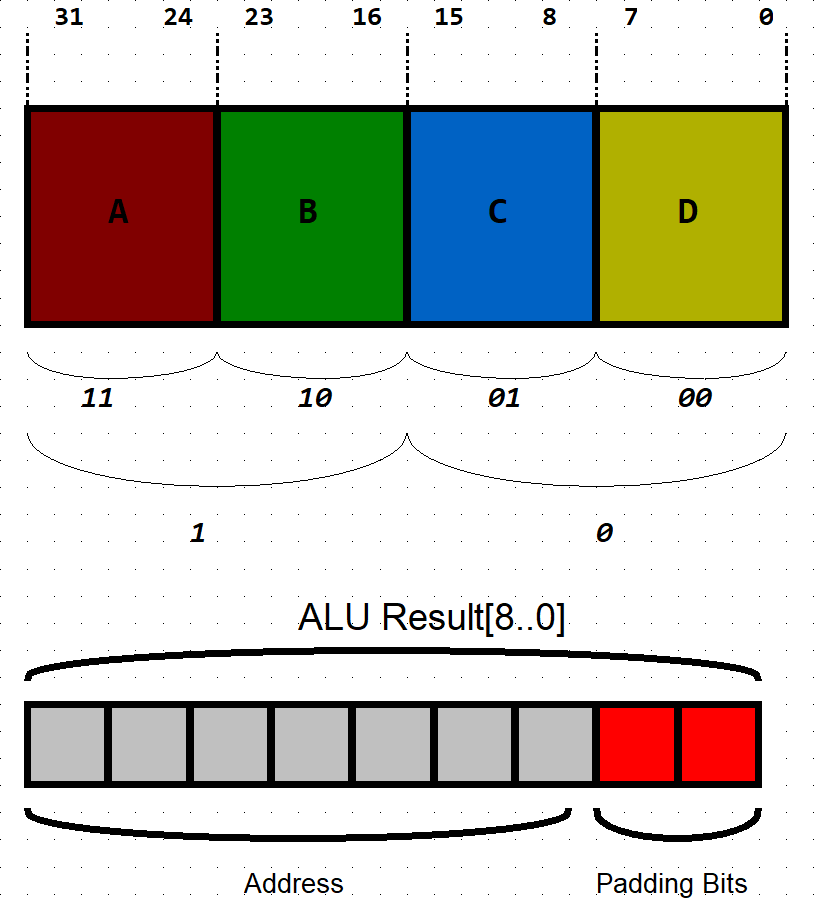
\includegraphics[width=0.5\textwidth]{PADDS}}
		\caption{Padding a D\$ Cell}
		\label{Image3.12}
	\end{center}
\end{figure}

\vspace{-2mm}

This introduction was mandatory to explain the functionality of the Byte Enable Module, which is dedicated to $STORE$ commands. It takes as input the value of the register $RS2$ and the two LSBs of the $ALU\_RES$ along with the three $MEMOP$ control bits, which represent the $STORE$ command type. Then according to the the value of the $MEMOP$ and the two LSBs, it generates the proper $BYTEEN$ signal.\footnote{ Refer to the \href{https://www.intel.com/content/dam/www/programmable/us/en/pdfs/literature/an/an207.pdf}{Altera's Internal Memory (RAM and ROM) User Guide} for further information about the Byte Enable option of the M4K Block} After the signal is generated then the module reforms $RS2$'s value according to the $STORE$ type. If the command is SB then the reformed word is \underline{$rs2[7..0] \ \& \ rs2[7..0] \ \& \ rs2[7..0] \ \& \ rs2[7..0]$}. If the command is SH then the reformed word is \underline{$rs2[15..0] \ \& \ rs2[15..0]$}. If the command is SW then word remains the same. This means that we can only write either the lowest byte or byte-half of the $RS2$ value if not all of it. Algorithm \ref{Algorithm3} demonstrates the behavior of Byte Enable Module;

\clearpage

\begin{algorithm}[H]
	\SetAlgoLined
	\SetKwInOut{Input}{input}\SetKwInOut{Output}{output}
	
	\Input{ $CONTROL\_WORD[2..0]$, $RS2\_VALUE[31..0]$ and $ALU\_RES[6..0]$}
	\Output{$BYTEEN[3..0]$ and $REFORMED\_RS2\_VALUE[31..0]$} 
	\BlankLine
	\BlankLine
	
	\emph{$MEMOP \leftarrow $ CONTROL\_WORD[1..0]}\;
	\emph{$PAD \leftarrow $ ALU\_RES[1..0]}\; 
	\emph{$BYTE \leftarrow $ RS2\_VALUE[7..0]}\;
	\emph{$HALF \leftarrow $ RS2\_VALUE[15..0]}\;
	
	\BlankLine
	/* Store Byte Case */ \\
	\BlankLine
	
	\uIf {MEMOP == "00"} 
	{
		\uIf 	{ PAD == "00"}{BYTEEN = "000\textbf{1}";}
		\uElseIf{ PAD == "01"}{BYTEEN = "00\textbf{1}0";}
		\uElseIf{ PAD == "10"}{BYTEEN = "0\textbf{1}00";}
		\uElseIf{ PAD == "11"}{BYTEEN = "\textbf{1}000";}
		\BlankLine
		\BlankLine
	    REFORMED\_RS2\_VALUE = BYTE \& BYTE \& BYTE \& BYTE; \footnote{: "$\&$" is the Concatenation Operator.}
	}
	\BlankLine
	/* Store Half Case */ \\
	\BlankLine
	
	\uElseIf {MEMOP == "01"}
	{
	
		\uIf	{ PAD[1] == "0"}{BYTEEN = "00\textbf{11}";}
		\uElseIf{ PAD[1] == "1"}{BYTEEN = "\textbf{11}00";}
		\BlankLine
		\BlankLine
		REFORMED\_RS2\_VALUE = HALF \& HALF; 
	}
	\BlankLine
	/* Store Word Case */ \\
	\BlankLine
	
	\uElseIf {MEMOP == "10"}
	{	
		BYTEEN = "\textbf{1111}"; \\
		REFORMED\_RS2\_VALUE = RS2\_VALUE; // No Modification\\
	}
	\uElse
	{
		BYTEEN = "XXXX"; 
	}
	
	
	\caption{Byte Enable Module Algorithm}
	\label{Algorithm3}
\end{algorithm}	
\vspace{2mm}


\subsection{\textcolor{orange}{Load Masking Module}}
\label{SubSec3.4.3:LMASK}

Besides the primary LW (Load Word) command, the RV32I ISA supports Signed and Unsigned Loads for Bytes and Halves, while the M4K memory block can only provide a word which is read from one of its memory cells. So we must design a circuit that will be responsible for making all those Load commands viable. The Load Masking Module is responsible for taking as input the word which has just been read from the D\$ and modifying accordingly as the Load type command instructs. The module was designed behaviorally and here is the algorithm that represents it:\\


\begin{algorithm}[H]
	{\footnotesize
	\SetAlgoLined
	\SetKwInOut{Input}{input}\SetKwInOut{Output}{output}
	
	\Input{ $CONTROL\_WORD[3..0]$, $MEMORY\_VALUE[31..0]$ and $ALU\_RES[1..0]$}
	\Output{$LOADED\_WORD[31..0]$} 
	
	\BlankLine
	\BlankLine
	
	
	\emph{$MEMOP \leftarrow  $ CONTROL\_WORD[1..0]}		  \;
	\emph{$PAD   \leftarrow  $ ALU\_RES}	  			  \; 
	\emph{$SIGNED/UNSIGNED \leftarrow $ CONTROL\_WORD[3]} \;
	\emph{$A \leftarrow MEMORY\_VALUE[31..24]$}\;
	\emph{$B \leftarrow MEMORY\_VALUE[23..16]$}\;
	\emph{$C \leftarrow MEMORY\_VALUE[15..8]$}\;
	\emph{$D \leftarrow MEMORY\_VALUE[7..0]$}\;
	
	\BlankLine
	/* Load Byte Case */
	\BlankLine
	\uIf {MEMOP == "00" } 
	{
		/* Signed */
		\uIf 	{ SIGNED/UNSIGNED == "0"}
		{
			\uIf 	{ PAD == "00"}{LOADED\_WORD = SE(MEMORY\_VALUE[7])  \& D; \footnote{: "SE" stands for Sign Extension.}}
			\uElseIf{ PAD == "01"}{LOADED\_WORD = SE(MEMORY\_VALUE[15]) \& C;}
			\uElseIf{ PAD == "10"}{LOADED\_WORD = SE(MEMORY\_VALUE[23]) \& B;}
			\uElseIf{ PAD == "11"}{LOADED\_WORD = SE(MEMORY\_VALUE[31]) \& A;}
		}
		/* Unsigned */
		\uElseIf{ SIGNED/UNSIGNED == "1"}
		{
			\uIf 	{ PAD == "00"}{LOADED\_WORD = ZF(MEMORY\_VALUE[31..8]) \& D; \footnote{: "ZF" stands for Zero Fill.}}
			\uElseIf{ PAD == "01"}{LOADED\_WORD = ZF(MEMORY\_VALUE[31..8]) \& C;}
			\uElseIf{ PAD == "10"}{LOADED\_WORD = ZF(MEMORY\_VALUE[31..8]) \& B;}
			\uElseIf{ PAD == "11"}{LOADED\_WORD = ZF(MEMORY\_VALUE[31..8]) \& A;}	
		}
		 
	}
	\BlankLine
	/* Load Half Case */
	\BlankLine
	\uIf {MEMOP == "01"}
	{	
		/* Signed */ \\
		\uIf {SIGNED/UNSIGNED == "0" }
		{
			\uIf 	{ PAD[1] == "0"}{LOADED\_WORD = SE(MEMORY\_VALUE[15]) \& CD;}
			\uElseIf{ PAD[1] == "1"}{LOADED\_WORD = SE(MEMORY\_VALUE[31]) \& AB;}
		}
		/* Unsigned */ \\
		\uElseIf{ SIGNED/UNSIGNED == "1" }
		{
			\uIf 	{ PAD[1] == "0"}{LOADED\_WORD = ZF(MEMORY\_VALUE[31..16]) \& CD;}
			\uIf 	{ PAD[1] == "1"}{LOADED\_WORD = ZF(MEMORY\_VALUE[31..16]) \& AB;}
		}
	}
	
	\uElse
	{	/* Load Word Case (Default) */\\
		LOADED\_WORD = MEMORY\_VALUE; 
	}
}
	
	
	\caption{Load Masking Module Algorithm }
	\label{Algorithm4}
\end{algorithm}	

\clearpage

\section{Write Back - WB}
\label{Sec3.5:WB}

The $Write \ Back$ stage is the final and simplest stage of our pipeline. Its the stage which signifies the completion of a command. It gathers the data that must be written to the command's $RD$ register (if any), along with the $RD$'s address and sends this information back to the Register File, which is located at the $ID$ stage.

\begin{figure}[h!]
	\begin{center}
		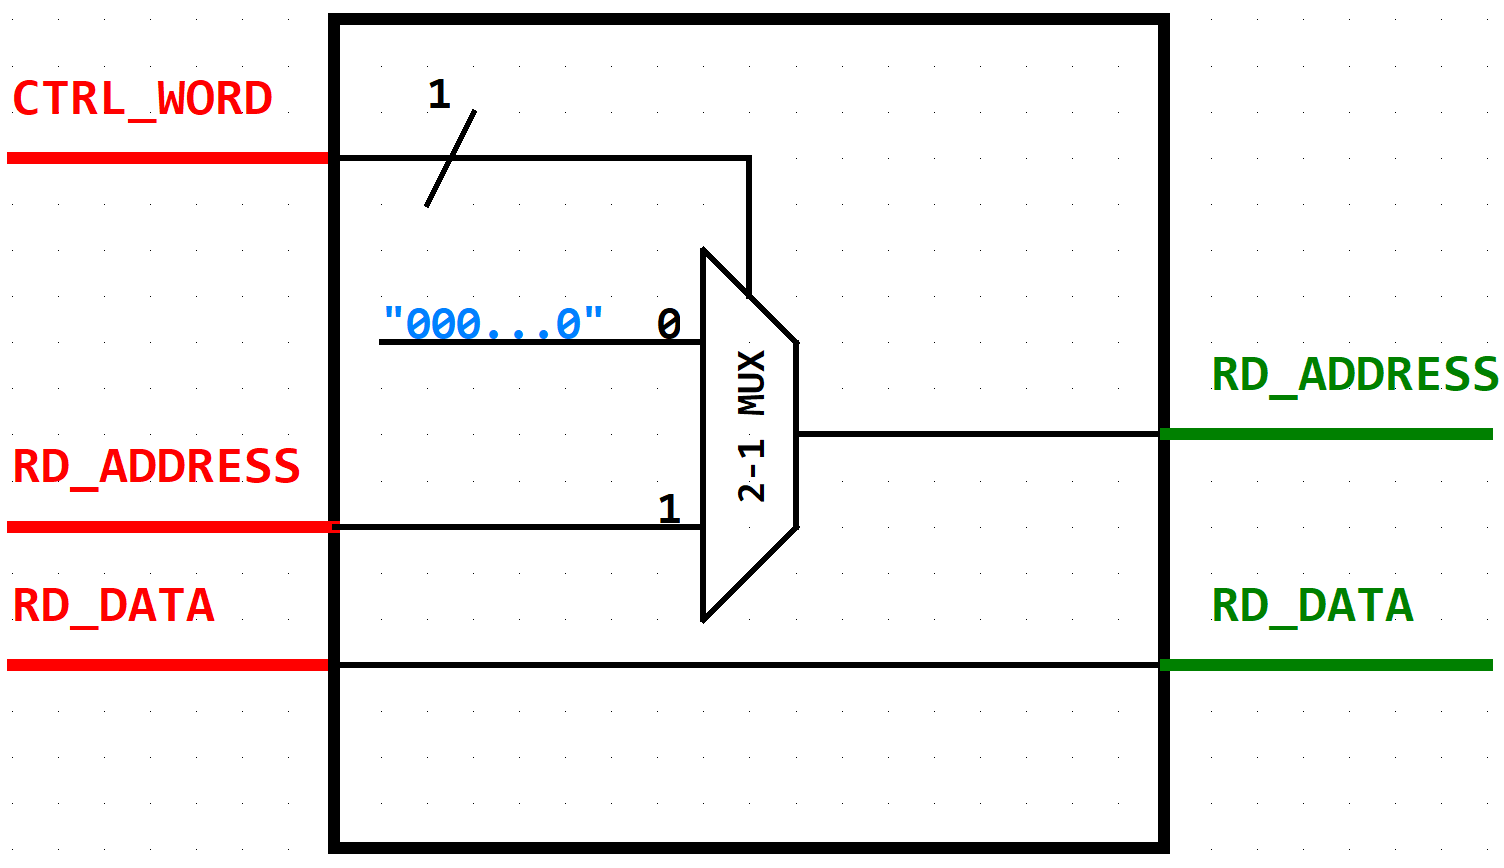
\includegraphics[width=0.75\textwidth]{WB}
		\caption{Write Back schematic}
		\label{Image3.13}
	\end{center}
\end{figure}

\vspace {-3mm}

The write back data can either be the result of the ALU if it is a computational command, or the result of the $MEM$ stage if it is a $LOAD$ command. Some commands, for example all the $STORE$s do not have a destination register so the $Write Back$ stage has no use. This is why we use a $2\rightarrow 1$ multiplexer, so for every instruction that has no $rd$ register we provide the address of the $x0$ register, which will do nothing since as we mentioned before the register $x0$ cannot be written and its hardwired to the constant $0$. The proper input of the multiplexer is selected by the control bit $WB\ OP$ which was previously generated at $ID$ stage.

\subsection{Forward Scenario D}
\label{SubSec3.5.1:FWDD}

Previously, at \hyperlink{page.22}{page 22} we analyzed the Forwarding/Bypassing paths of our pipeline. We covered Forward of type A,B and C. But there is one extra forwarding that must happen when we encounter the following Scenario;

\begin{lstlisting}[caption={Forward Path D Example},captionpos=b]
OP_A	Reg_X, Reg_A, Reg_B
....	.....  .....  .....
....	.....  .....  .....
OP_B 	Reg_Y, Reg_X, Reg_C
\end{lstlisting}

This forward path is being handled by some external, pipeline logic that does not belong to the $Stall \ and \ Forwarding \ Predictor \ Module$ of the $ID$ stage. Normally this would not be an issue if we could write and then instantly read from the same register inside the Register File. But when we tested the full design without the Forward Path D, we confronted some data corrupt cases since in some tests the Write and Read of the same register were successful and in others were not.

\section{The Complete Pipeline}
\label{Sec3.6:COMPLETE}

We presented with great detail the five basic stages of our system. In this section we will analyze the complete pipeline of the RV32I ISA, and all the components that were previously mentioned as external/pipeline modules. Also we will discuss about the peculiarity of the M4K memory blocks and how they were a "problem" to our initial design plans. \\

Lets begin by introducing the extra, yet mandatory components for a pipeline architecture; the pipeline registers. Shown in Figure \ref{Image3.14} there are four registers (A/B/C/D) one for each data transaction between the CPU modules. They were implemented using behavioral architectures based on the standard D flip flop logic. All four registers have a reset $RST$ \footnote{It is used to initialize the whole system.}signal (the same signal we mentioned for the previous modules) which is positive edge triggered and occurs when the CPU starts working (on clock cycle \#0). All registers have as many inputs as the number of output signals the previous\footnote{For example Pipeline Register A has two data inputs (I\$ WORD and PC VALUE).}CPU module provides, plus some signals that are transfered from one stage to the next one \footnote{For example, in $EXE$ stage there are two signals transfered directly to register C from register B (RD ADDRESS and RS2 VALUE).}. Registers A and B have also two extra control signals, the $FLUSH$\footnote{ Empties all the data the register currently has. }  and $STALL$ signals which occur every time we encounter a RAW hazard ($STALL$) and whenever we have a conditional or unconditional jump case ($FLUSH$). \\

Furthermore, there is one extra register, the $PC$ (Instruction Pointer), which is a simple 32-bit register that holds the memory address of the next instruction that would be fetched. After providing the address to $IF$ module its value gets updated accordingly:
\vspace{2mm}
\begin{itemize}
	\item Either provides the address of the next instruction ($PC+4$).
	\item Or in case of Jump/Branch provides the target address of the Jump.
\end{itemize}
\vspace{2mm}
Secondly,  we will make it easy for one to navigate into Figure \ref{Image3.14} since it has a lot of detail and it may seem confusing. So we will begin by pairing colors to the respective purposes and functionalities that they bespeak: 
\vspace{2mm}
\begin{itemize}
	\item The $PC$ register and the next PC signal ($NPC$) are drawn with \textcolor{purple}{\textbf{purple}} color.
	\item Figure's \ref{Image3.4} color code for forwarding paths (FWD \textcolor{forestgreen(web)}{\textbf{A}}/\textcolor{bred}{\textbf{B}}/\textcolor{azure}{\textbf{C}}/\textcolor{citrine}{\textbf{D}}) is the same in Figure \ref{Image3.14}.
	\item The $STALL$ and $FLUSH$ control signals are depicted with \textcolor{ao}{\textbf{deep blue}} color.
	\item The $CONTROL\_WORD$ and all its forks are depicted with \textcolor{orange}{\textbf{orange}} color.
	\item The $CLOCK$ and $RST$ signals are depicted with \textcolor{burgundy}{\textbf{dark red}} color.
\end{itemize}
\vspace{2mm}

Lastly, there are three extra pipeline modules that we created to make the signal distribution and the workload for every stage less and easier. These modules are the \textcolor{olive}{ALU INPUT SELECTOR}, the \textcolor{orange}{CONTROL WORD REGROUP} module and the \textcolor{burgundy}{WB SELECTOR} respectively.
\clearpage
\begin{figure}[h!]
	\begin{center}
		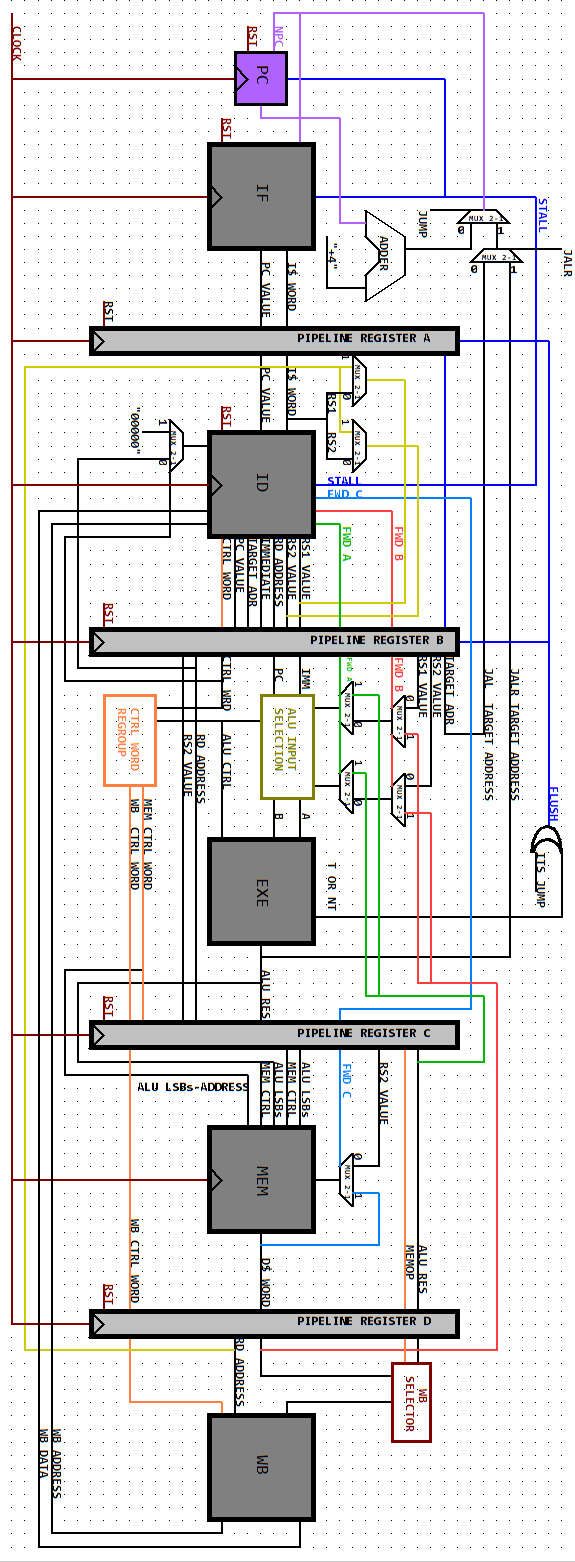
\includegraphics[height=0.98\textheight, width=0.98\textwidth]{RV32I}
		\caption{RV32I schematic}
		\label{Image3.14}
	\end{center}
\end{figure}
\clearpage

\subsection{\textcolor{olive}{ALU Input Selector}}
\label{SubSec3.6.1:ALUIN}

The $EXE$ stage which has the Arithmetic and Logic Unit, simply requires two operands and one control word to operate. The problem here is that there are many different commands in our ISA which require different operations and different operands, hence we should either attach more circuitry to the $ID$ module (which is already overloaded with functions) or design an outer-pipeline stage module dedicated for this work, which is what we finally chose. \\

The ALU Input Selector module takes as input the $RS1$ and $RS2$ values from the Register File, the $PC$ and $IMMEDIATE$ from the $ID$ stage, along with some control bits, the $JALR$, $JUMP$, $PC$ and $IMM$ \footnote{Redirect to \hyperlink{page.18}{page 18} for more information about the meaning of the control bits.} and decides according to the following schematic which are going to be operands A and B that will finally go to the $EXE$ stage.
 
\begin{figure}[h!]
	\begin{center}
		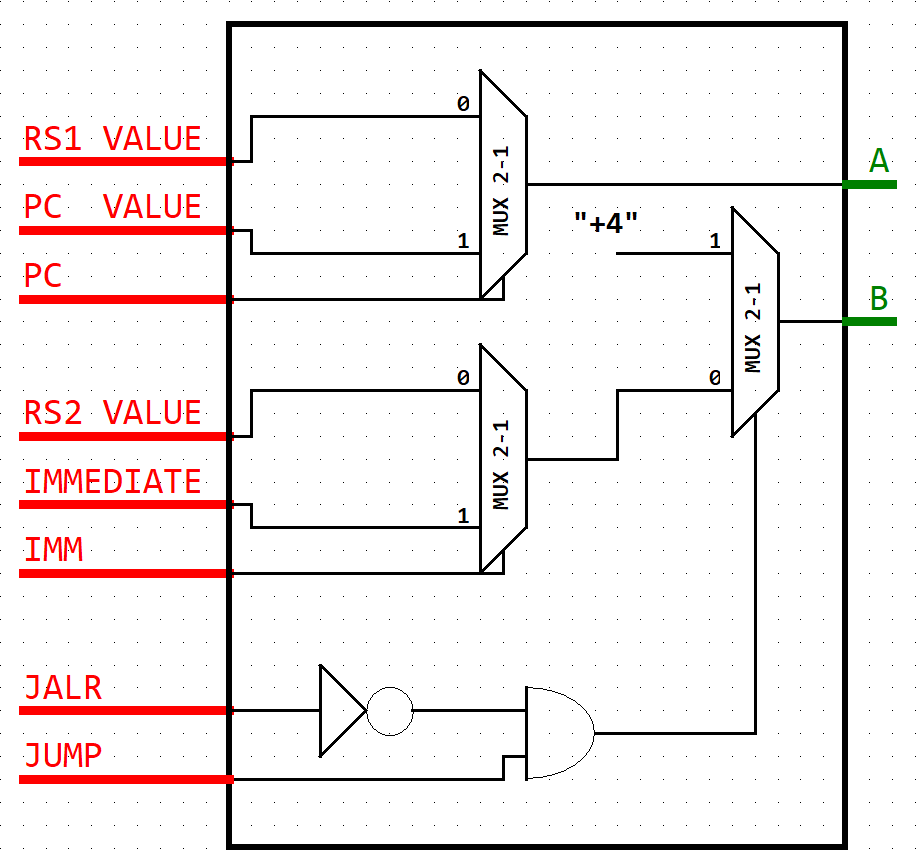
\includegraphics[width=0.75\textwidth]{ALU_INPUT_SELECTOR}
		\caption{ALU Input Selector schematic}
		\label{Image3.15}
	\end{center}
\end{figure}

The first two $2\rightarrow1$ multiplexers are selecting either the $RS1/2$ values or their alternatives, which for $RS1$ is the $PC$ value ( the commands that do not have an $RS1$ register in their type, e.g "AUIPC" ) and for $RS2$ is the $IMMEDIATE$ that is generated at $ID$ ( the commands that do not have an $RS1$ register in their type, e.g "ADDI" ). The inputs are selected by the corresponding control bits. The third $2\rightarrow1$ multiplexer is used to implement the theory we developed at sub-section \ref{SubSec3.2.5:ADDER}, in which we segregate the work of the $ID$'s Adder and $EXE$'s ALU that has to be done in $JALR$ and $JAL$ cases.
\clearpage

\subsection{\textcolor{orange}{Control Word Regroup Module}}
\label{SubSec3.6.2:CTRLWRDRGRP}	

As we indicated before, the $ID$ stage generates a control-word which is necessary for the following pipeline stages, since it dictates which operations they must undertake. This control-word though, is large and its not completely useful in every stage. To facilitate our design we designed the Control Word Regroup Module which given the control-word which was generated from $ID$, it divides it into smaller ones which are addressed to the respective pipeline stages. It also provides the essential control bits to the ALU Input Selector module. The module's behavioral architecture is described by the following simple algorithm:\\


\begin{algorithm}[H]
	\SetAlgoLined
	\SetKwInOut{Input}{input}\SetKwInOut{Output}{output}
	
	\Input{ $CONTROL\_WORD[17..0]$}
	\Output{$ALU\_SELECTOR\_WORD[3..0]$, $ALU\_CONTROL\_WORD[8..0]$, $MEM\_AND\_WB\_CONTROL\_WORD[4..0]$}
{\footnotesize 	\BlankLine
	\BlankLine
	/* Bits for ALU Selector */ \\
	\emph{$JALR \leftarrow $ CONTROL\_WORD[0]}\;
	\emph{$JUMP \leftarrow $ CONTROL\_WORD[2]}\; 
	\emph{$PC   \leftarrow $ CONTROL\_WORD[3]}\; 
	\emph{$IMM  \leftarrow $ CONTROL\_WORD[4]}\; 
	\BlankLine
	/* Bits for ALU */ \\
	\emph{$SHIFT/ADDER/LOGIC \ OP \leftarrow $ CONTROL\_WORD[12..11]}\;
	\emph{$ALU \  OP 		 		\leftarrow $ CONTROL\_WORD[10..9]}\;
	\emph{$INV \ LOGIC 			\leftarrow $ CONTROL\_WORD[8]}\;
	\emph{$EQ||LT				\leftarrow $ CONTROL\_WORD[7]}\;
	\emph{$BRANCH		 	 	\leftarrow $ CONTROL\_WORD[6]}\;
	\emph{$SLT			 	 	\leftarrow $ CONTROL\_WORD[5]}\;
	\emph{$LUI		 	 		\leftarrow $ CONTROL\_WORD[1]}\;
		
	\BlankLine
	/* Bits for MEM and WB */ \\
	\emph{$MEM \ U \ OP	 	 		\leftarrow $ CONTROL\_WORD[16]}\;
	\emph{$MEM \ OP 				\leftarrow $ CONTROL\_WORD[15..13]}\;
	\emph{$WB \ OP				\leftarrow $ CONTROL\_WORD[17]}\;
	\BlankLine}
	\BlankLine
	
{\footnotesize 	\emph{{\footnotesize $ALU\_SELECTOR\_WORD\leftarrow JALR$ $\&$ $JUMP$ $\&$ $PC$ $\&$ $IMM$}}\;
	\emph{{\footnotesize $ALU\_CONTROL\_WORD  \leftarrow SHIFT/ADDER/LOGIC \ OP$ $\&$ $ALU \ OP$ $\&$ $INV \ LOGIC$ $\&$ $EQ||LT$ $\&$ $BRANCH$ $\&$ $SLT$ $\&$ $LUI$}}\;
	\emph{{\footnotesize $MEM\_AND\_WB\_CONTROL\_WORD \leftarrow MEM \ U \ OP$ $\&$ $MEM \ OP $ $\&$ $WB \ OP$}}\;
	\caption{Control Word Regroup}}
	\label{Algorithm5}
\end{algorithm}	
\vspace{2mm}

We do not separate at this point further the control-word for $MEM$ and $WB$ stages because they have many bits in common. The separation will occur later inside the pipeline registers.

\subsection{\textcolor{burgundy}{WB Selector}}
\label{SubSec3.6.3:WBSEL}
This module is actually a $2\rightarrow1$ multiplexer which decides if the value that must be written back to the Register File's $RD$ register should be the result from $EXE$'s ALU or $MEM$'s D\&. This is done by and-reducing the control-bits of $MEMOP$, and selecting with it either the ALU result (if the result is 1) or the D\$ read word (if the result is 0):

 \begin{center}
	$\mathbf{if}$$ \ (MEMOP[2] \land MEMOP[1] \land MEMOP[0])' == \mathbf{1 \rightarrow D\$\_WORD}$ \\
	$\mathbf{if}$$ \ (MEMOP[2] \land MEMOP[1] \land MEMOP[0])' == \mathbf{0 \rightarrow ALU\_RES}$ \\
\end{center}

\clearpage

\subsection{The M4K Block Issue}

The memory type of our caches is the M4K block. We chose this type of memory, because we wanted our design to be fully synthesizable and since we have already worked with Altera's DE-2 FPGA board, this is the only memory we could use and actually test. But with this selection, a design problem appeared; these memory blocks, have by default registered inputs and optionally registered outputs. This means, for stages $IF$ and $MEM$, who have the caches embedded into the, that for every instruction that passes through them we would need two clock cycles and not one, as we initially had planned.

\begin{figure}[h!]
	\begin{center}
		\fbox{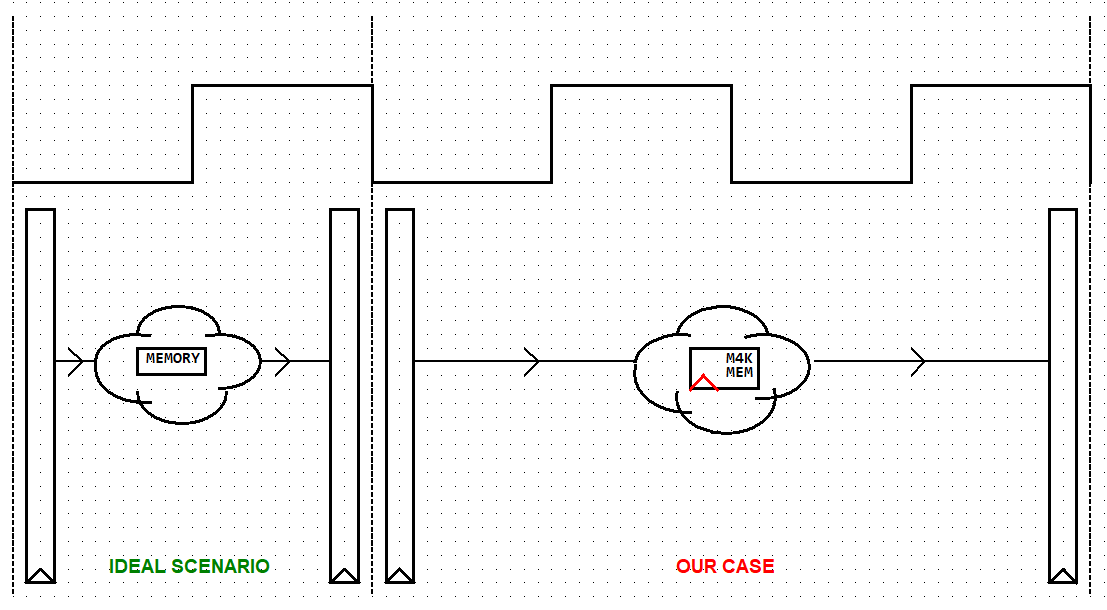
\includegraphics[width=1\textwidth]{M4KPROB}}
		\caption{Design problem due to the M4K blocks.}
		\label{Image3.17}
	\end{center}
\end{figure}

So, for the $ID$ and $MEM$ pipeline stages, we had to figure out a solution to this problem; having 2 clock cycles for some pipeline stages and one clock cycle for the rest, was considered unacceptable by us. The plan is for every pipeline stage to be operative in 1 clock cycle. So, we simply ignored the $PC$ register in the case of $IF$ stage and we ignored the $PIPELINE \ REGISTER \ C$ in the case of $MEM$ stage. So every signal that is directed either towards the I\$ or the D\$ is coming directly from another module and not from a register.

\begin{itemize}
	\item For $IF$ which has the I\$ the signal that skips the $PC$ register is the Next Pc Value ($NPC$), which is used as address.
	\item For $MEM$ which has the D\$ the signals that skip the Pipeline Register C are:
	\begin{itemize}
		\item The control-bits which concern the $STORE$ commands.
		\item The $RS2$ register value which concerns the $STORE$ commands.
		\item The LSB's from the ALU, which are used as offset.		
		\item The $ALU\_RES[8..2]$ which is used as address.
	\end{itemize}	
\end{itemize}



  	